\documentclass[runningheads]{thesis/latex/llncs}
\usepackage[T1]{fontenc}
\usepackage{listings}
\usepackage{graphicx}
\usepackage[inline]{enumitem}
% hide link border
\usepackage[hidelinks]{hyperref}
% reset section numbering in chapters
\usepackage{bookmark}
\bookmarksetup{
  numbered,
  open
}

% BigO
\usepackage{fourier}
\DeclareMathAlphabet{\mathcal}{OMS}{cmsy}{m}{n}
\SetMathAlphabet{\mathcal}{bold}{OMS}{cmsy}{b}{n}
\newcommand{\bigO}{\mathcal{O}}

\usepackage{csquotes}
% Allow sub-figures
\usepackage{subcaption}

\usepackage[acronym]{glossaries}
\makeglossaries
\newacronym{acl}{ACL}{access control list}
\newacronym{acp}{ACP}{access control policies}
\newacronym{as}{AS}{authorization server}
\newacronym{cern}{CERN}{European Organization for Nuclear Research}
\newacronym{css}{CSS}{Community Solid Server}
\newacronym{dom}{DOM}{Document Object Model}
\newacronym{dns}{DNS}{Domain Name Server}
\newacronym{dpop}{dpop}{Demonstrating Proof-of-Possession}
\newacronym{ess}{ESS}{Enterprise Solid Server}
\newacronym{html}{HTML}{Hypertext Markup Language}
\newacronym{hsts}{HSTS}{\gls{http} Strict Transport Security}
\newacronym{http}{HTTP}{Hypertext Transfer Protocol}
\newacronym{https}{HTTPS}{\gls{http} Secure}
\newacronym{idp}{IDP}{identity provider}
\newacronym{iri}{IRI}{Internationalized Resource Identifier}
\newacronym{js}{JS}{JavaScript}
\newacronym{ldp}{LDP}{Linked Data Platform}
\newacronym{ldpc}{LDPC}{Linked Data Platform Container}
\newacronym{ldpr}{LDPR}{Linked Data Platform Resource}
\newacronym{mit}{MIT}{Massachusetts Institute of Technology}
\newacronym{mvp}{MVP}{minimum viable product}
\newacronym{nhs}{NHS}{National Health Service}
\newacronym{nss}{NSS}{Node Solid Server}
\newacronym{oidc}{OIDC}{OpenID Connect}
\newacronym{poc}{POC}{proof of concept}
\newacronym{rdf}{RDF}{Resource Description Framework}
\newacronym{rdfs}{RDFS}{\gls{rdf} Schema}
\newacronym{ro}{RO}{resource owner}
\newacronym{rs}{RS}{resource server}
\newacronym{sla}{SLA}{service level agreement}
\newacronym{solidoidc}{Solid OIDC}{Solid OpenID Connect}
\newacronym{solidos}{SolidOS}{Solid operating system}
\newacronym{sso}{SSO}{single sign-on}
\newacronym{sts}{STS}{Solid Test Suite}
\newacronym{ts}{TS}{TypeScript}
\newacronym{uk}{UK}{United Kingdom}
\newacronym{uri}{URI}{Uniform Resource Identifier}
\newacronym{wac}{WAC}{Web Access Control}

% \usepackage[acronym]{glossaries}
% \newacronym{acl}{ACL}{access control list}
\newacronym{acp}{ACP}{access control policies}
\newacronym{as}{AS}{authorization server}
\newacronym{cern}{CERN}{European Organization for Nuclear Research}
\newacronym{css}{CSS}{Community Solid Server}
\newacronym{dom}{DOM}{Document Object Model}
\newacronym{dns}{DNS}{Domain Name Server}
\newacronym{dpop}{dpop}{Demonstrating Proof-of-Possession}
\newacronym{ess}{ESS}{Enterprise Solid Server}
\newacronym{html}{HTML}{Hypertext Markup Language}
\newacronym{hsts}{HSTS}{\gls{http} Strict Transport Security}
\newacronym{http}{HTTP}{Hypertext Transfer Protocol}
\newacronym{https}{HTTPS}{\gls{http} Secure}
\newacronym{idp}{IDP}{identity provider}
\newacronym{iri}{IRI}{Internationalized Resource Identifier}
\newacronym{js}{JS}{JavaScript}
\newacronym{ldp}{LDP}{Linked Data Platform}
\newacronym{ldpc}{LDPC}{Linked Data Platform Container}
\newacronym{ldpr}{LDPR}{Linked Data Platform Resource}
\newacronym{mit}{MIT}{Massachusetts Institute of Technology}
\newacronym{mvp}{MVP}{minimum viable product}
\newacronym{nhs}{NHS}{National Health Service}
\newacronym{nss}{NSS}{Node Solid Server}
\newacronym{oidc}{OIDC}{OpenID Connect}
\newacronym{poc}{POC}{proof of concept}
\newacronym{rdf}{RDF}{Resource Description Framework}
\newacronym{rdfs}{RDFS}{\gls{rdf} Schema}
\newacronym{ro}{RO}{resource owner}
\newacronym{rs}{RS}{resource server}
\newacronym{sla}{SLA}{service level agreement}
\newacronym{solidoidc}{Solid OIDC}{Solid OpenID Connect}
\newacronym{solidos}{SolidOS}{Solid operating system}
\newacronym{sso}{SSO}{single sign-on}
\newacronym{sts}{STS}{Solid Test Suite}
\newacronym{ts}{TS}{TypeScript}
\newacronym{uk}{UK}{United Kingdom}
\newacronym{uri}{URI}{Uniform Resource Identifier}
\newacronym{wac}{WAC}{Web Access Control}

% \newglossaryentry{data pod}
{
  name=data pod,
  description={is a place for storing documents, with mechanisms for controlling who can access what.}
}
\newglossaryentry{Solid app}
{
  name=Solid app,
  description={is an application that reads or writes data from one or more data pods.}
}
\newglossaryentry{thing}
{
  name=Thing,
  description={is a data entity, e.g., a person. A Thing is associated with a set of data or properties about the Thing, e.g., name, date of birth, address, etc.}
}
% \makeglossaries

\usepackage[sorting=none]{biblatex}
\addbibresource{thesis/latex/bibliography.bib}

\usepackage{float}
\usepackage{upquote}
\usepackage{fancyvrb}
\usepackage{color}
\usepackage[legalpaper, margin=1in]{geometry}

% use for newline after paragraph
\newcommand{\emptybox}[2][\textwidth]{%
  \begingroup
  \setlength{\fboxsep}{-\fboxrule}%
  \noindent\framebox[#1]{\rule{0pt}{#2}}%
  \endgroup
}

% set left,right padding for table
\setlength{\tabcolsep}{10pt}
% set top,bottom padding for table
\renewcommand{\arraystretch}{1.25}

%% Save the class definition of \subparagraph
\let\llncssubparagraph\subparagraph
%% Provide a definition to \subparagraph to keep titlesec happy
\let\subparagraph\paragraph
%% Load titlesec
\usepackage[compact]{titlesec}
%% Revert \subparagraph to the llncs definition
\let\subparagraph\llncssubparagraph

% hide chapter numbering on new chapter page
\titleformat{\chapter}[display]{\normalfont\bfseries}{}{0pt}{\LARGE}

% make paragraph bold
\titleformat*{\paragraph}{\itshape\mdseries\bfseries}

% Minted code highlighting
% \usepackage{thesis/latex/minted}

% colors for code snippets
\definecolor{commentscolor}{rgb}{0.5,0.5,0.5}
\definecolor{greenstrings}{rgb}{0,0.5,0}
\definecolor{backgroundgray}{rgb}{0.95,0.95,0.95}

\lstset{escapeinside={(*@}{@*)}}
\lstdefinelanguage{Other}%
{ sensitive=true,
  numbers=left,
  backgroundcolor = \color{backgroundgray},
  stepnumber=1,
  basicstyle=\ttfamily,
  breaklines=true,
  xleftmargin=\parindent,
  aboveskip=\bigskipamount,
  tabsize=2,
  morecomment=[l][\color{commentscolor}]{///},
  morecomment=[l][\color{commentscolor}]{//},
  morecomment=[s][\color{commentscolor}]{{(*}{*)}},
  morestring=[b]",
  showstringspaces=false,
  literate={`}{\`}1,
  stringstyle=\color{greenstrings},
  basicstyle=\small,
}

\setcounter{tocdepth}{3}
% numbering on subsubsection
\setcounter{secnumdepth}{3}
\begin{document}
\begin{titlepage}
   \begin{center}
       \vspace*{1cm}
       \Huge
       \textbf{CERN-Solid Code Investigation}\\
       \LARGE
       \vspace{0.5cm}
        Proof of Concept, Challenges, and Continuation\\
        
       \vspace{1cm}
       
       \normalsize
        by\\
        
       \vspace{1cm}
       
       \Large
       \textbf{Jan Schill}\\
        schi@itu.dk
        
       \vfill
       
       \normalsize
        Supervisors:\\
        
       \vspace{0.3cm}
       
       \textbf{Philippe Bonnet} (ITU)\\
        phbo@itu.dk
        
       \vspace{0.3cm}
       
       \textbf{Maria Dimou} (CERN)\\
        maria.dimou@cern.ch
        
       
       \vspace{1cm}
       
        A thesis presented for the degree of\\
        Master of Science
        
       \vspace{1cm}
       
        Course code: KISPECI1SE
        
       \vspace{0.5cm}
       
       
\includegraphics[width=0.4\textwidth]{thesis/latex/assets/university.jpg}
       
       Computer Science\\
       IT University of Copenhagen\\
       Denmark\\
       01.06.2021
            
   \end{center}
\end{titlepage}

\tableofcontents
\newpage
\chapter{Introduction}
% \setcounter{section}{0}
\section{Context}

The Web was created in 1989 by Sir Tim Berners-Lee while working at the institution of \gls{cern} “\textelp{} to allow people to work together by combining their knowledge in a web of hypertext documents” \cite{timbl-bio}. This brilliant idea has ever since grown as an essential part of our all lives \cite{cern-solid-investigation-spec}. While bringing a new platform for innovation into existence, a new level of oppression and surveillance that has never been seen before has facilitated without most even realizing. Data are harvested and analyzed to generate models describing and predicting human behavior far beyond what is morally tolerable. These actions permit the generation of large amounts of wealth as capitalistic and governmental bodies enjoy a great interest in these models to either generate more profit or more control. The escalation of attraction towards data has led to the construction of so called \textit{data silos}, where data gatherers built attractive applications for users while locking them into their walled gardens to have the all data for themselves and then selling it.

Through whistle blowing, active journalism, and technical education a new wave of hope is arising in the ocean of data hunting. Not giving up on the Web, which has in its little over 30 years of lifetime proven its paramount act in state, society, and the economy, Sir Tim has an adjustment for the Web specified. With the help of several Web enthusiasts, companies, and even governments the idea of Solid was found.

Solid aims at giving the users back the control over their data to regain full data sovereignty. It does so by specifying through a number of technical reports a new way of building application in the Web that let the users control their data and in this way can decide who can see what. Just like the Web, which was also defined by technical reports and prototypes, it is for everyone and not limited by anything. 

“Being the Web’s birthplace, \gls{cern} remains a High Energy Physics laboratory; hence, its primary mission is to run an accelerator, its detectors, and the relevant experiments. Computing is of paramount importance for filtering, storing, distributing, accessing, analyzing the experimental data. Nevertheless, due to its large and distributed user base, \gls{cern} offers sophisticated solutions on all software application fronts. In terms of price and transparency, proprietary packages have been disappointing. Following the raising worldwide awareness of personal data ownership and sovereignty, \gls{cern} is interested in Solid.” \cite{cern-solid-investigation-spec}

\section{Goal}

\newpage
\chapter{Related Work}
% \setcounter{section}{0}

This chapter will hold the parts of the project coming from the outside, all the relevant efforts happening in the Solid Community or \gls{cern}'s involvement in the collaboration.

\section{Background}

The \textit{\gls{cern}-Solid Code Investigation} project aims at linking \gls{cern} with Solid. Some of this linkage has been done forming a status quo check of the Solid ecosystem in \cite{cern-solid-investigation-spec}. This previous work and the efforts around the two \glspl{poc} shall give insights into a symbiosis of \gls{cern} and Solid.

The following sections in this chapter will introduce the two systems and their significant subsystems, modules, libraries, or techniques. 

\section{Indico}

Indico is one of CERN’s most sophisticated software projects. It is an event management tool, giving users a means to organize complex meetings or conferences with an easy-to-use interface. It was started in 2002 as a \textit{European project} and has been in production at CERN ever since. It is used daily to facilitate more than 600,000 events at CERN. It has helped others like the UN “to put in place an efficient registration and accreditation workflow that greatly reduced waiting times for everyone” at conferences with more than 180,000 participants in total \cite{cern-solid-investigation-spec}.

\subsection{Events}

Being an event management tool at Indico's core lies the \texttt{Event} class. The Event's \gls{ui} is presented in \ref{fig:indico-event-interface}, showing all sorts of attachable information. 

\begin{figure}[H]
    \centering
    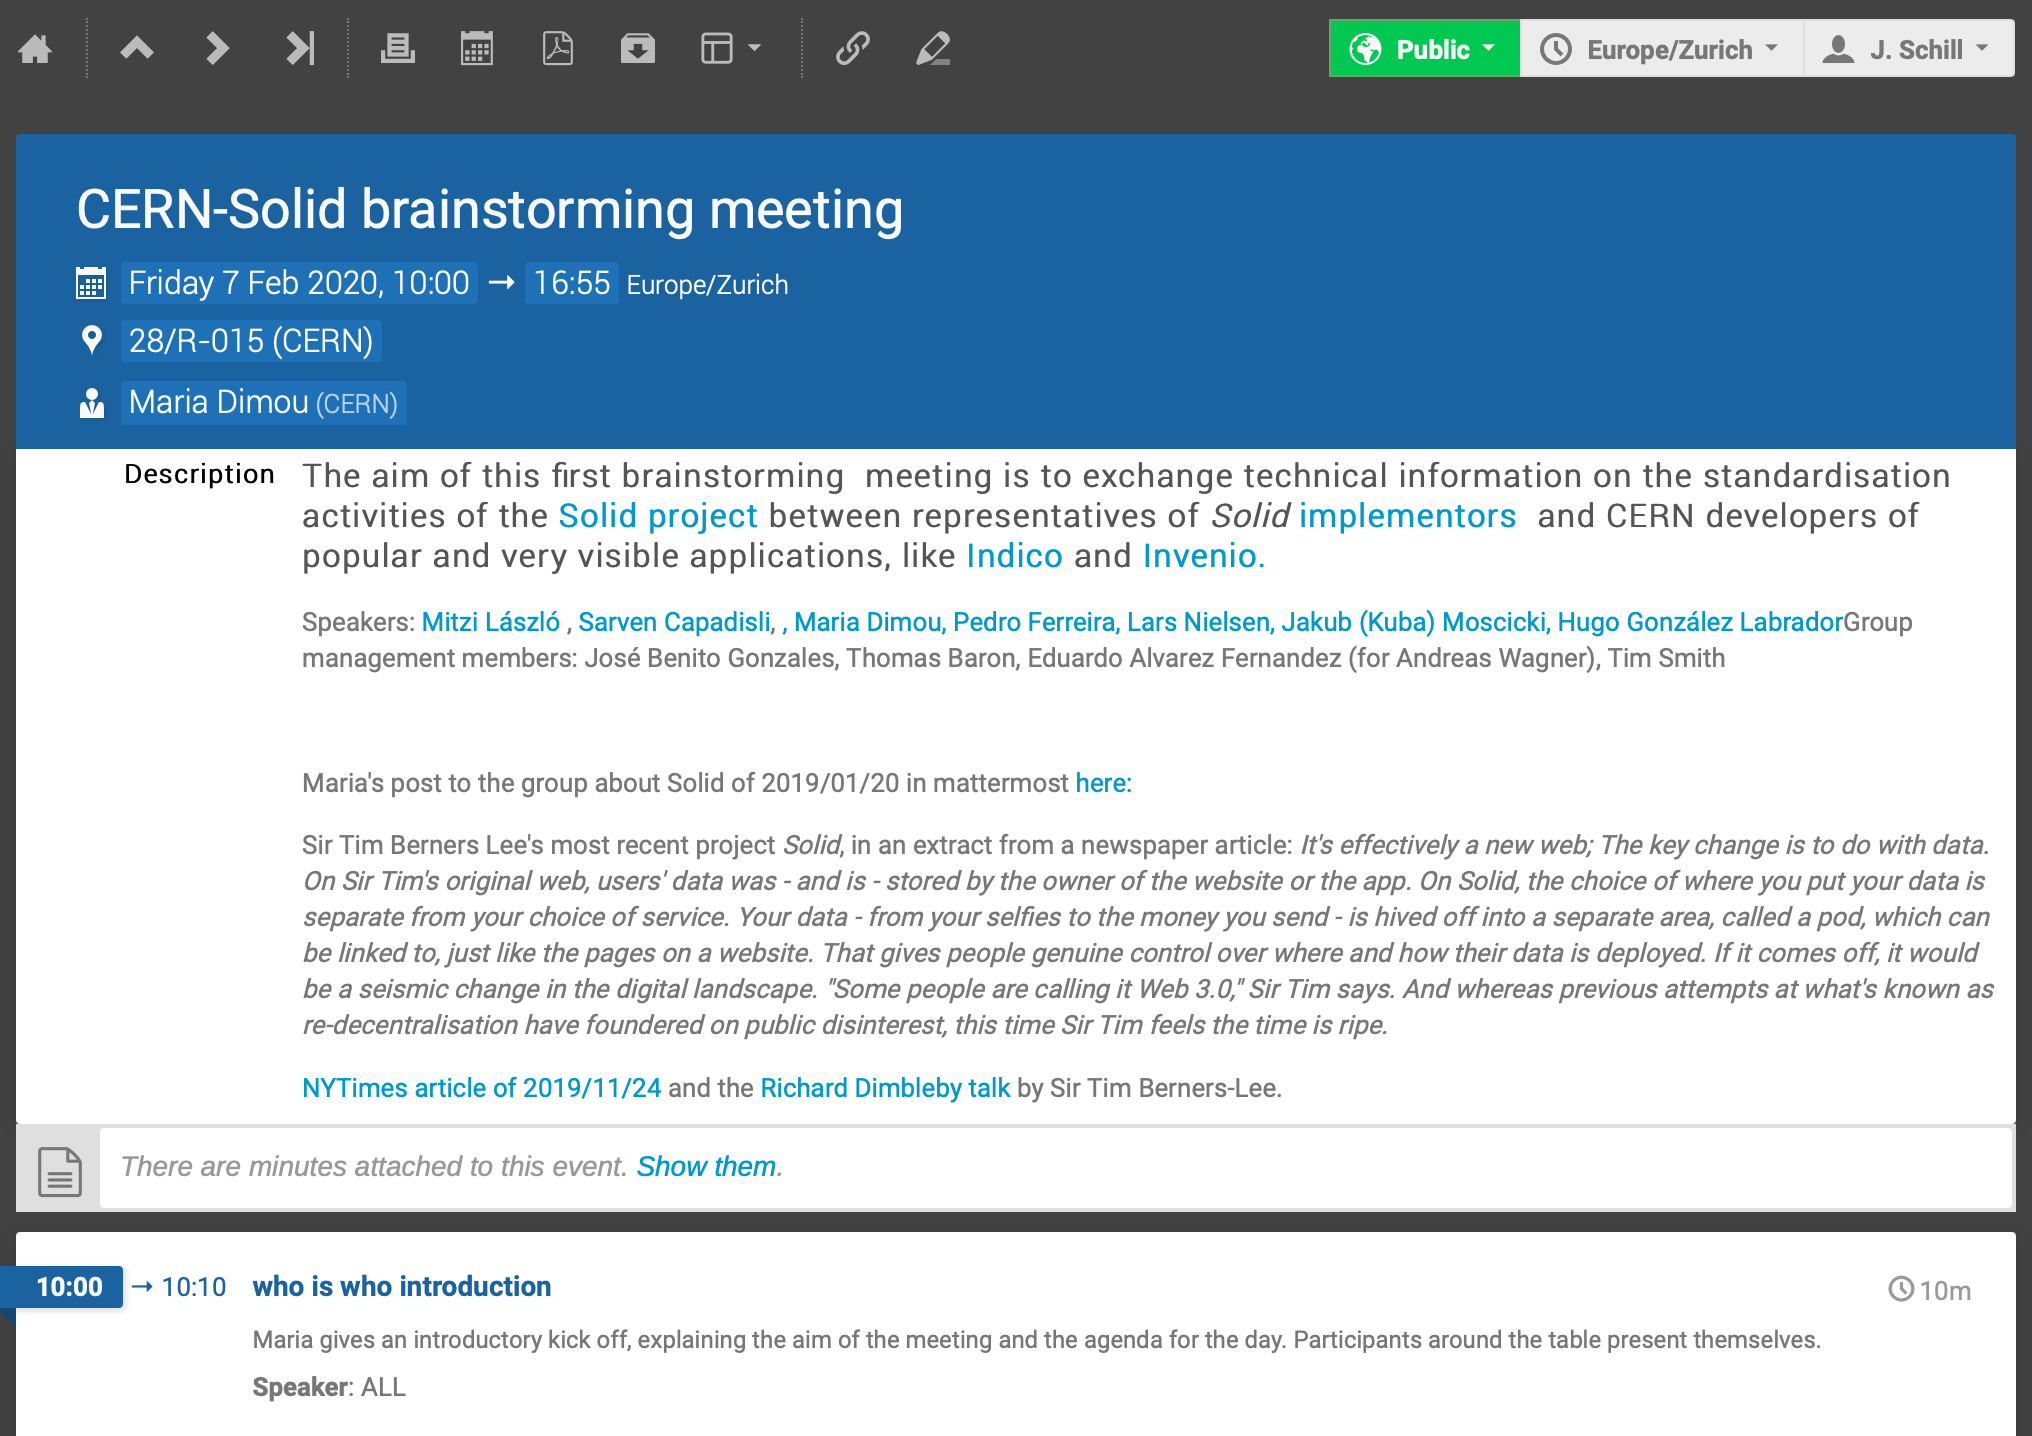
\includegraphics[width=0.6\textwidth]{thesis/latex/assets/indico-event-interface.png}
    \caption{\gls{ui} of an Indico event.}
    \label{fig:indico-event-interface}
\end{figure} 

\subsection{Storage Mechanisms}

All events, all information in these events, file uploads, everything put into Indico are stored in a relational database on centralized servers. \gls{cern}'s Indico instance is hosted on-premise in their own data centers. Another crucial feature of Indico is the permanent archival of event material and metadata \cite{cern-indico}. It allows lifetime access to all events hosted on the platform. As an example, one can easily browse to the event "Big Data and Social Media" held by Vint Cerf in 2018 \cite{vint-cerf} and have access to description, recording, and slides, or even a presentation given in 2004 about "Practical Use of XML" \cite{titov}.

\subsubsection{EventSettingsProxy}\mbox{}\\

A \textit{proxy class} enables storage for event-specific settings. Commonly stored data types are contact email addresses for an event. In Indico these \texttt{EventSettingsProxy} are stored in a database table called \texttt{settings}. Adding a new \texttt{setting} for the \gls{poc}, it will receive a field in the row specific to the event.

\subsection{Conferences}

In Indico, an event can be simple meetings, lectures, or all kinds of presentations. Additionally, Indico allows the creation and management of conferences. Conferences are more complex events with several more features, including registration, call-for-abstracts, program definition, payments, and more \cite{cern-indico-docs}. The conference registration is especially interesting for this project as it is part of the \gls{poc}.

\subsubsection{Conference Registration}\mbox{}\\

Once a conference is created, the conference manager needs to make a registration form to allow signups to the event. This form is created in Indico's backend and has default personal information fields but can be expanded as much as needed with free text fields. Payment for participation also needs to be enabled in this step. Meaning, as soon as a user fills in all the mandatory information and submits it, a successfully finished payment prompt will only complete the registration.

\section{Solid}

An initial introduction to Solid was given as part of a previous \textit{research project} \cite{cern-solid-investigation-spec} in preparation for this thesis. In the \textit{research project}, the Solid specification was, among other things, summarized and analyzed. This section will reiterate and study the subsequent experiment-relevant parts further.

\subsection{Authentication With Solid}

In the Solid ecosystem, agents identify themselves with their WebID and prove their ownership through the \gls{solidoidc} protocol, a flavor of \gls{oidc}. For further explanation and flow diagrams through the authentication process, see either the work done in the previous report \cite{cern-solid-investigation-spec} or the \gls{solidoidc} specification itself \cite{solid-ecosystem-oidc}.

To help with the complex authentication flow of \gls{solidoidc} a few libraries have been developed by different actors. Two libraries relevant for this project exist; their relevancy is discussed in the chapter \ref{chapter:investigation} under the section \ref{subsubsection:design}.

\begin{table}[h!]
    \centering
    \begin{tabular}{| l | l | l |} 
     \hline
     Name & Solid Auth Fetcher & solid-client-authn \\
     \hline
     Repository URL & \url{github.com/solid/solid-auth-fetcher} & \url{github.com/inrupt/solid-client-authn-js} \\
     \hline
     Language & \gls{ts} & \gls{ts} \\
     \hline
     Maintainer & Solid Community & Inrupt \\
     \hline
     Last updated & 2021/03/05 & 2021/05/12 \\
     \hline
    \end{tabular}
    \vspace{0.75cm}
    \caption{Two Solid authentication libraries.}
    \label{table:0}
\end{table}

Solid Auth Fetcher is a fork of the \texttt{solid-client-authn} developed by Inrupt but has not seen much development recently. With the quickly evolving Solid ecosystem, it is vital to have working and up-to-date libraries to build applications in this ecosystem. Both libraries are similar in their core functionality, and both support authenticating with the latest Solid servers, and thus the choice is not as important. Still, the frequency of commits in Inrupt's repository indicates a more active development and a more reliable source when problems arise. This way, one does not rely on support from open-source developers, which is, per se, not a bad thing.

For this simple reason, the programming of the \gls{poc} where Solid authentication was needed was enabled through Inrupt's \texttt{solid-client-authn}.

\subsection{Reading and Writing Linked Data}

Data in Solid is stored as Linked Data \cite{Malhotra:15:LDP}. \gls{rdf} is a framework for representing Linked Data information in the Web \cite{Cyganiak:14:RCA}. The default file format implemented by the existing Solid servers is \textit{Turtle} \cite{Prud:hommeaux:14:RT}.

The graph-based data model from using \gls{rdf} also requires additional computation as it is not natively supported with helper functions in \gls{js}, such as \gls{json}. The benefit of using \gls{json} in \gls{js} is that a \gls{json} object is automatically parsed as an object and can be operated on by using the dot notation to access attributes of the \gls{json} data structure. For \gls{rdf}, this is not the case for an into the program loaded Turtle resource.

Fortunately, existing libraries come to the rescue allowing such operations on the \gls{rdf}-based data type. Again Inrupt and the Solid Community offer solutions. For the same reasons, it was decided to use Inrupt's solution for this development as it acts as a convenient wrapper to the bare bone Linked Data \gls{api} implemented in \texttt{rdflib.js} \cite{rdflib-js}. Even though working with \gls{rdf} can be quickly done using \texttt{rdflib.js}, Inrupt's libraries tie nicely together and allow, for instance, a seamless passing of an authenticated session to its client library to enable authenticated requests to protected resources.

As mentioned before and looked at in detail in \cite{cern-solid-investigation-spec}, the Turtle format is a graph data structure built up with triplets---a triplet statement in its simplest form a sequence of (subject, predicate, object) terms \cite{Prud:hommeaux:14:RT}. 

Inrupt decided to call this construct a \texttt{Thing}, a data entity associated with a set of data or properties of this \texttt{Thing} \cite{inrupt-thing}. A \texttt{SolidDataset} is a set of things \cite{inrupt-dataset}.

The following code listing shows how to use helper methods to extract data from a Turtle file loaded by sending a request to the WebID profile document \gls{uri}.

\begin{lstlisting}[language=Other,columns=fullflexible, caption={Basic usage of Inrupt's solid-client library.}, label={lst:2}]
// Import statements omitted for this demonstration
// 1
const myDataset = await getSolidDataset(
  "https://janschill.net/profile/card"
);
// 2
const myProfile = getThing(
  myDataset,
  "https://janschill.net/profile/card#me"
);
// 3
const fn = getStringNoLocale(myProfile, VCARD.fn);
// fn => "Jan Schill"
\end{lstlisting}

\begin{enumerate}
    \item \textbf{Fetching the Turtle resource at the given \gls{uri}}: Notice here the WebID profile document \gls{uri} is being loaded, referring to the document describing the agent behind the WebID \gls{uri}.
    \item \textbf{Loading triplet statement into a variable}: Now, the actual triplet statement containing information behind this specific agent is mapped to the \texttt{myProfile} variable.
    \item \textbf{Reading a value from a triplet}: Every subject and predicate is a \gls{uri}. The subject here is the loaded profile from the WebID \gls{uri} and the to be extracted value from the statement matching on the subject and predicate. When evaluated, the predicate \texttt{VCARD.fn} returns a \gls{uri}, which on dereferencing describes what kind of value can be obtained from the object.
\end{enumerate}

\subsection{Authorization Through WAC}

The as per Solid specification decided authorization mechanism is through \gls{wac} \cite{wac}. The majority of Solid servers use \glspl{acl} to manage the access modes on containers and resources. An \gls{acl} contains all the users and their permitted access rights to the resources on the pod. It may include a \textit{default}, or \textit{public} entry but must contain a reference to who the owner is to what the \gls{acl} is describing. \glspl{acl} are convenient as they allow easy and fast access to who has access to a specific resource. In contrast, \textit{capability tickets} are the preferred technique when finding out what a particular user has access to \cite{stallings}.

\subsection{Application Launcher}

A so-called \textit{application launcher} can mitigate a later presented discovery of a flaw in assigning unnecessary full access controls. The inconvenience lies in the fact when an application asks the client for what the allowed scope to its data pod is, most often, complete access control on the root container is needed -- this is against the security principle or tactic called \textit{least privilege}. The least privilege means to give actors of a system only exactly as much access they need and never more. The reason why this finds its way into the \glspl{poc} will be presented in the chapter \ref{chapter:investigation}.

For now, an implementation shall be introduced showing how the application launcher can avoid this problem. When an application wants to create \glspl{acl} on a data pod, it needs the before-mentioned \textit{control} access. \textit{Control} access is the highest access mode in \gls{wac}. An agent with \textit{control} access can read, write, and modify \gls{acl} resources -- meaning the owner of files can be changed as an example.
In the initial \gls{solidoidc} flow, one step asks for the application's allowed access scope. The asked for scope is for the root container of the data pod -- a more fine-grained control to limit access on a specific child container does not exist. An application launcher is a Solid app that has full control of the pod and must be trusted. When a new application wants use a data pod and needs control access but could, in theory, be limited to a specific container, the application launcher will create the appropriate \gls{acl} files to only allow precisely this.
This works because all access modes are defined in \gls{acl} files, which can be dynamically created. The application will, with this launcher, now have complete control of the container it operates and stores data in but cannot reach outside of its container.

The source code for a standalone application launcher in \gls{js} exists here \cite{app-launcher}.

\newpage
\chapter{Investigation}\label{chapter:investigation}
% \setcounter{section}{0}

\section{Proof of Concepts}

One main part of the investigation into the CERN-Solid collaboration is the development of a \gls{poc}. The \gls{poc} contains the creation of two independent software modules in an existing system from \gls{cern}. These software modules should show how it is to develop with the Solid principles in mind and to the Solid standard.

The goal of these modules is the symbiosis of decentralized stored data in a highly functional system without comprising its performance, security, or usability.

\subsection{POC 1: Commenting Module for Events in Indico}

The first \gls{poc} is supposed to enrich the Indico system with some sort of Solid-based content. With the product owner and chief developer of Indico, the CERN-Solid project manager and a Solid developer it was decided a commenting module for Indico events is an adequate solution to include data from an external storage entity namely a data pod. The ability to allow users of Indico to leave a comment on an event, which then lives in a data pod completely controlled by the author of the comment was concluded to be an attractive feature for Indico.

\begin{figure}
    \centering
    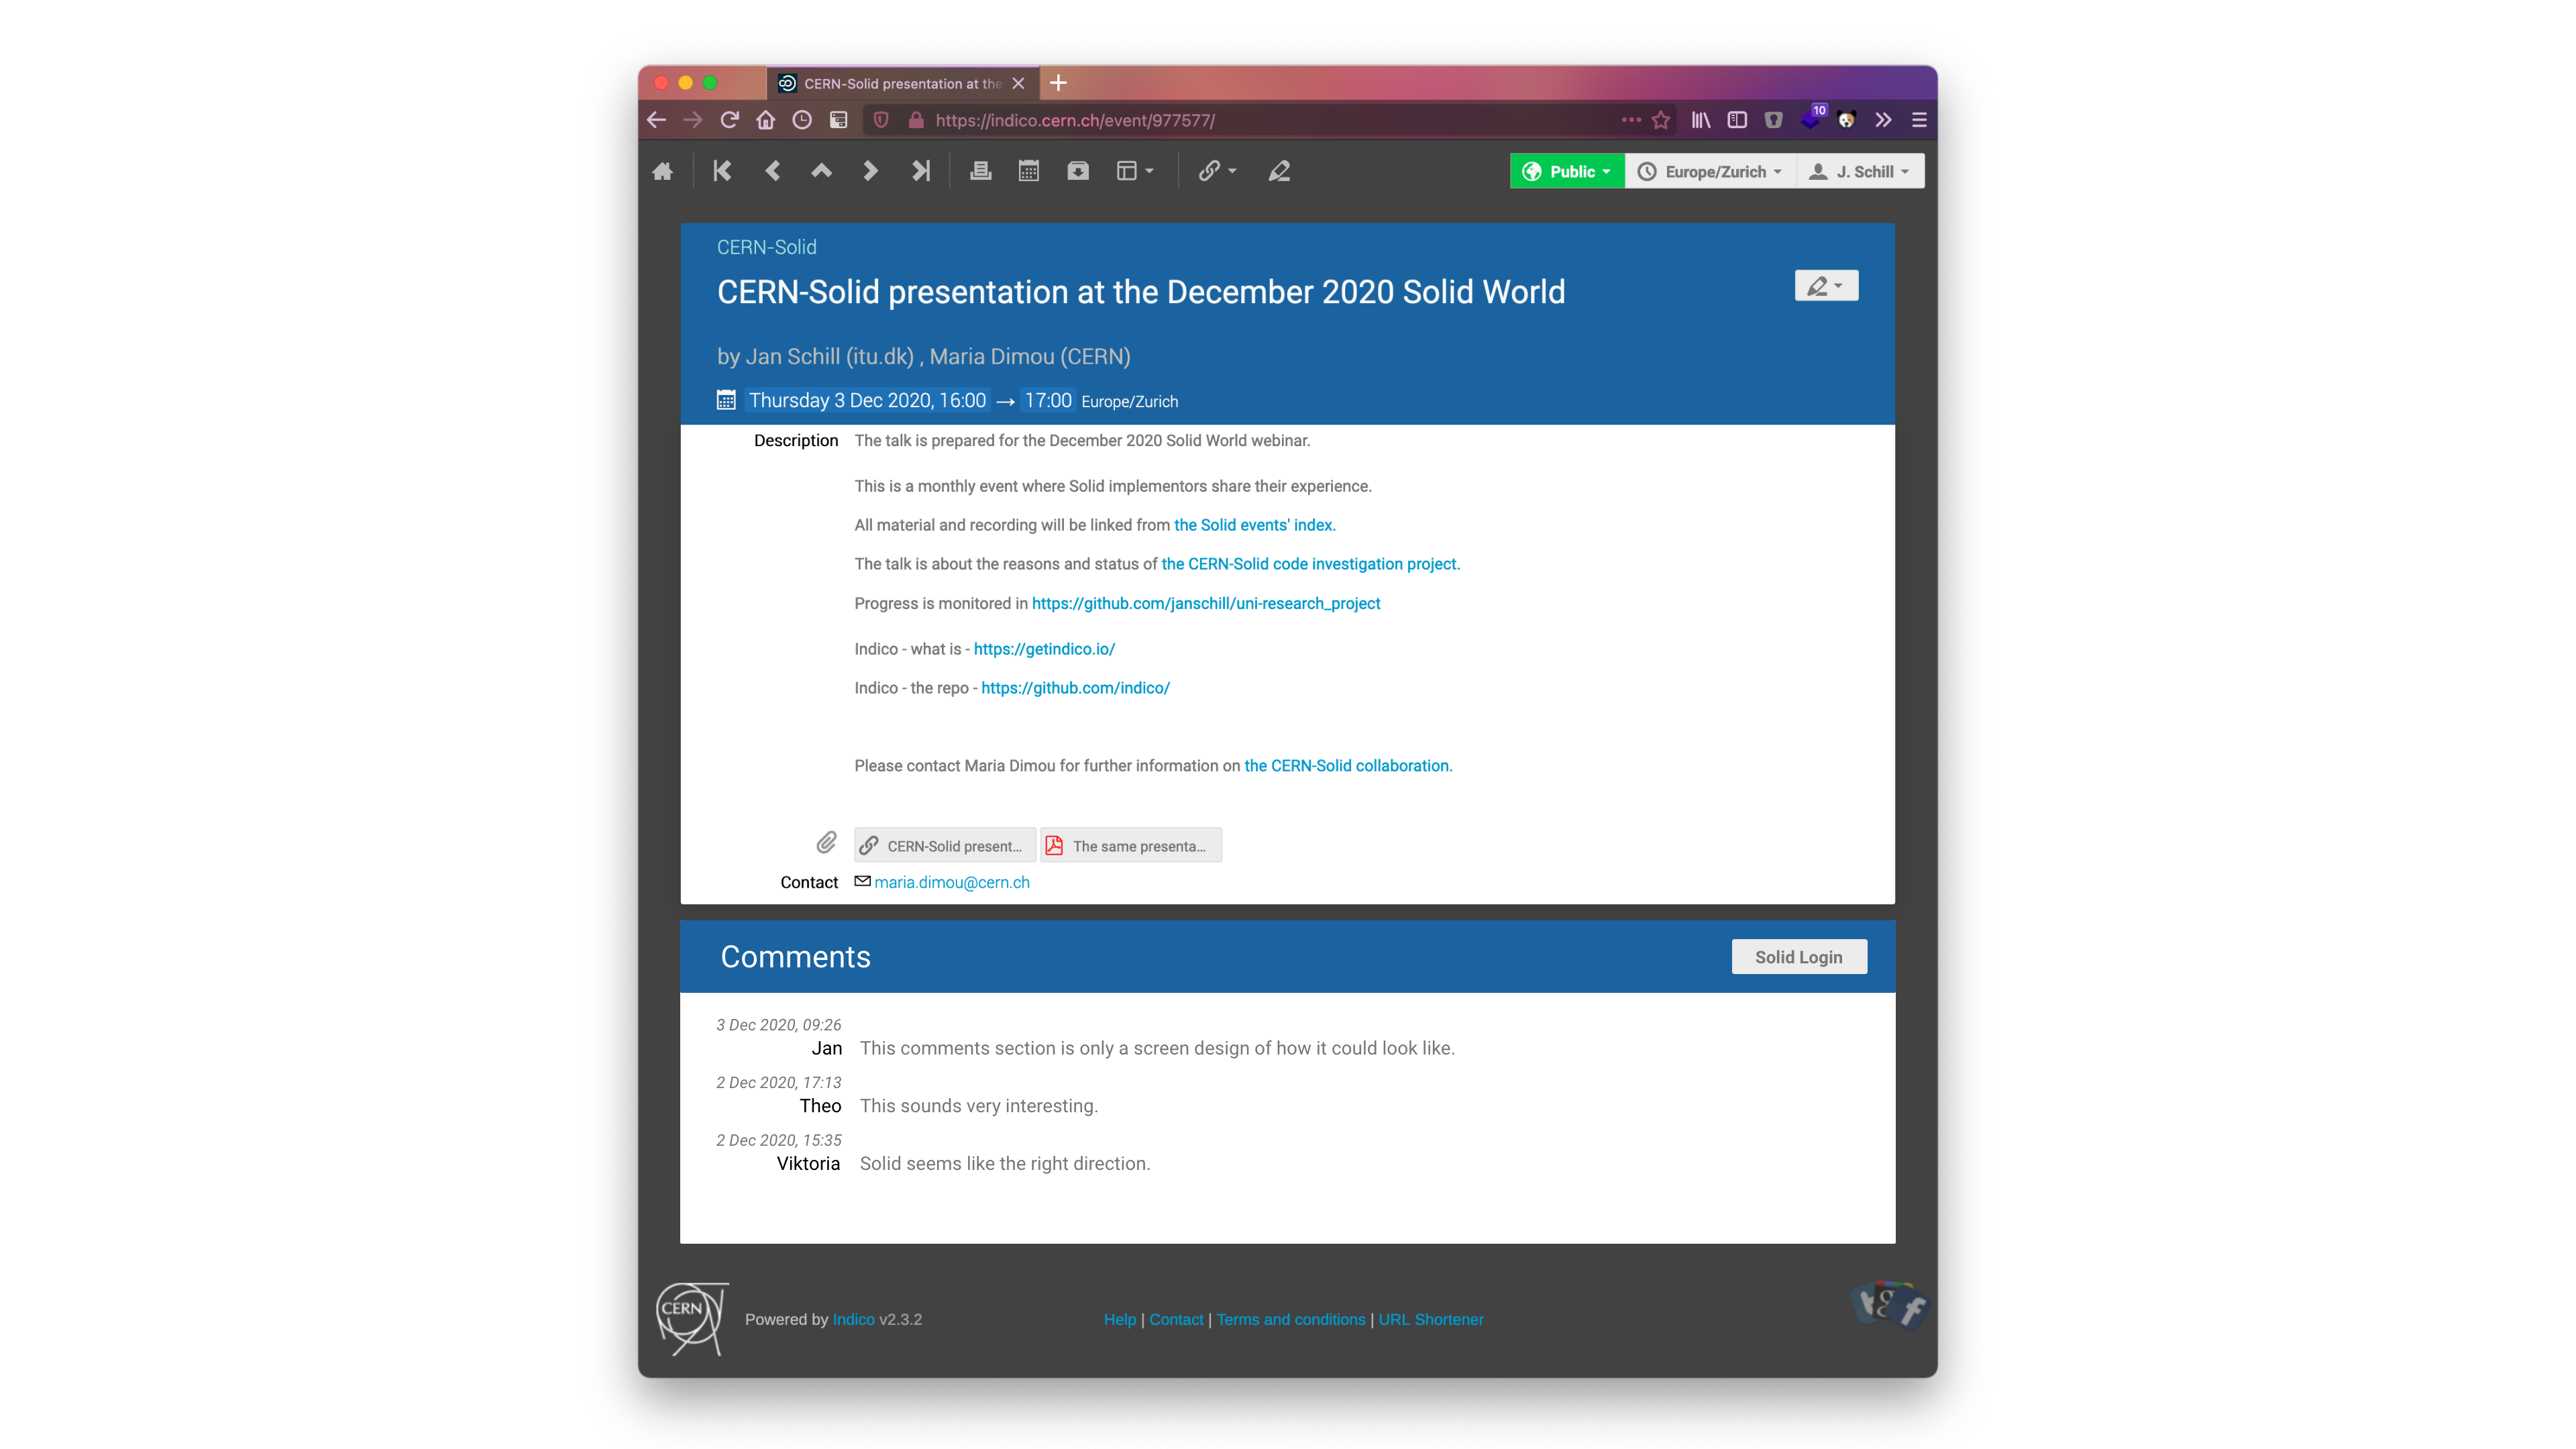
\includegraphics[width=1\textwidth]{prototype/screen_design/indico-comments-screen_design.png}
    \caption{User interface showing the comment module.}
    \label{fig:indico-comments-screen_design}
\end{figure}

\subsubsection{Design}\mbox{}\\

For the implementation of this module several design decisions had to be made. From the fundamental choice of the module running on the client device or be computed on the server and then propagated to the client afterwards or even with a microservice proxying all traffic through it to enable Solid without changing Indico.
Other design challenges were around how to protect the resources holding the comment information. These resources reside on the external data pod and need to be fetched from the application and read by other agents. Can \glspl{acl} be configured to allow the specific use-case?

\paragraph{Client- Versus Server-Side Versus Microservice}\mbox{}\\

When an agent browses to a running instance of Indico most of the functionality is being prepared on the server hosting Indico. It retrieves the specific request, builds the \gls{html}, and sends it to the user. For Indico most of the functionality is built with Python and the web framework Flask. Sometimes functionality needs to be closer to the user, an example is dynamic rendering of \gls{dom} elements. This is useful when new data needs to be shown right away without getting the blank white screen on a page reload.
Indico does send JavaScript, which is used for client-side features, but it focuses on keeping most its features on the server.

To make the right decision if the module should be primarily developed for the client- or server-side or even as a microservice, a list of requirements to the module had to be defined. With the defined requirements in place it had to be figured out how much functionality can be extracted from existing libraries and how much needed to be implemented with the new module. Implementing existing functionality for a new programming language would defeat the \gls{poc}’s purpose of showing how an existing software could work with the Solid principles.

The rudimentary set of features to enable commenting for users in Indico while saving the data in a data pod includes: 

\begin{enumerate}
    \item Authentication with a Solid \gls{idp}
    \item (Authenticated) Requests to a data pod
    \item Parsing of structured data (Linked Data)
\end{enumerate}

\paragraph{Client Approach}\mbox{}\\

The module runs in the browser and is therefore written in JavaScript. A programming language which compiles to JavaScript, such as TypeScript, is also possible. This means Indico remains mostly untouched, but would have to serve the needed JavaScript to the client on traffic to an event endpoint where the comment module is integrated.

\begin{table}[h!]
    \centering
    \begin{tabular}{| l | l |} 
     \hline
     Problem & Solution \\
     \hline
      Language & JavaScript or TypeScript  \\
      Framework & Native JavaScript  \\
      Client & solid-client-js \cite{solid-client-js}  \\
      Authentication & solid-client-authn-browser \cite{solid-client-authn-browser} \\
      RDF & solid-common-vocab-js \cite{solid-common-vocab-js}, rdflib.js \cite{rdflib.js}  \\
     \hline
    \end{tabular}
    \vspace{0.75cm}
    \caption{Existing solutions to problems for a client approach.}
    \label{table:1}
\end{table}

The communication flow with the data pod and the module would happen primarily from the browser.

\begin{figure}[H]
    \centering
    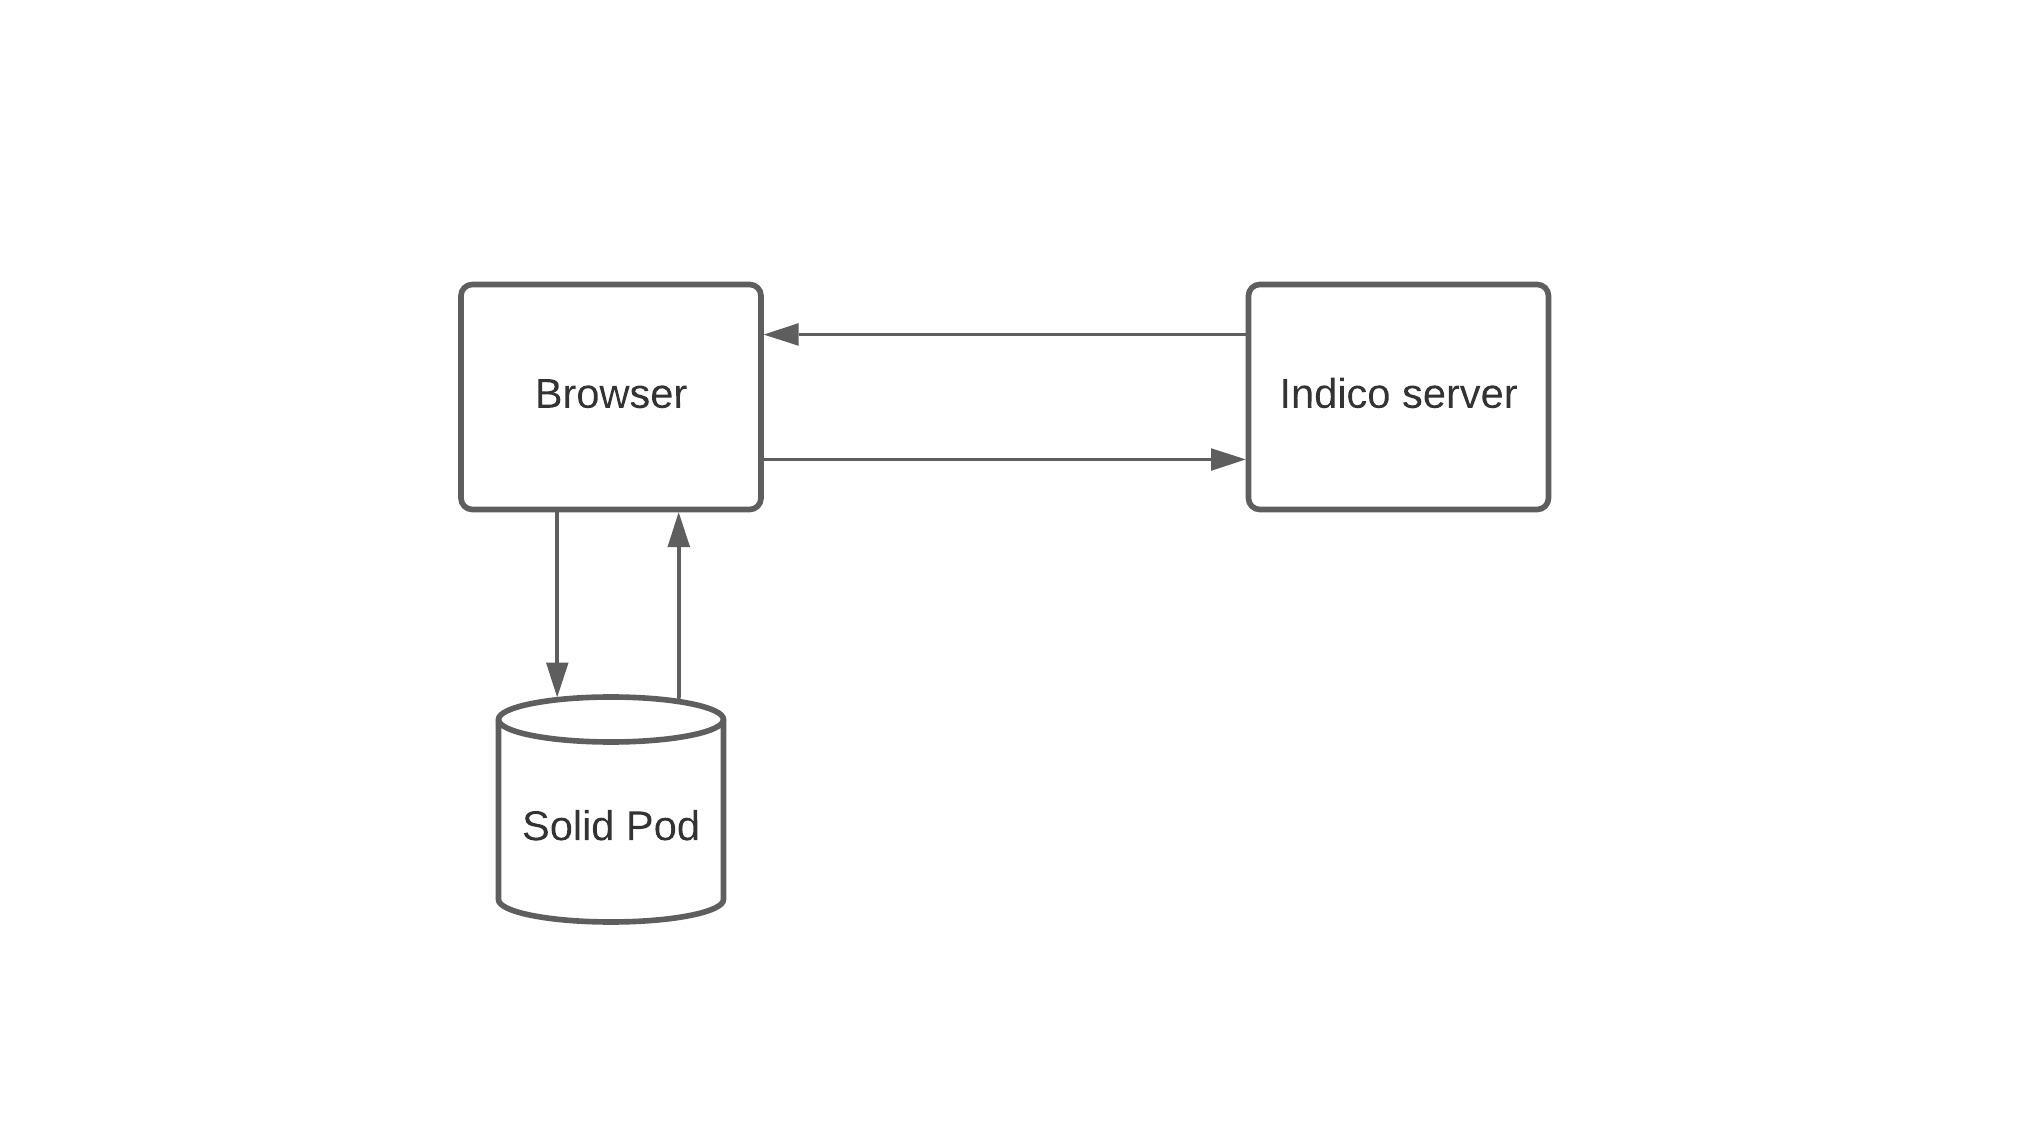
\includegraphics[width=0.8\textwidth]{prototype/graphs/poc-infrastructure-frontend.jpeg}
    \caption{Communication flow for a module developed on the client.}
    \label{fig:poc-infrastructure-frontend}
\end{figure}

\paragraph{Microservice Approach}\mbox{}\\

The microservice approach would allow developing the needed Solid logic on a separate service, which proxies all Solid related traffic through it an enable the Solid functionality. Most of the libraries from the client implementation can be used as well, as both developments would be written in JavaScript. Only the authentication flow would work a bit different.

\begin{table}[h!]
    \centering
    \begin{tabular}{| l | l |} 
    \hline
     Problem & Solution \\
     \hline
      Language & JavaScript or TypeScript  \\
      Framework & Node.js  \\
      Client & solid-client-js \cite{solid-client-js}  \\
      Authentication & solid-client-authn-node \cite{solid-client-authn-node} \\
      RDF & solid-common-vocab-js \cite{solid-common-vocab-js}, rdflib.js \cite{rdflib.js}  \\
    \hline
    \end{tabular}
    \vspace{0.75cm}
    \caption{Existing solutions to problems for a microservice approach.}
    \label{table:2}
\end{table}

The microservice module would handle take all requests aimed at the data pod and make it compliant with the Solid server. It would provide the client with the proper \gls{solidoidc} flow to attach the access token to all authenticated requests.

\begin{figure}[H]
    \centering
    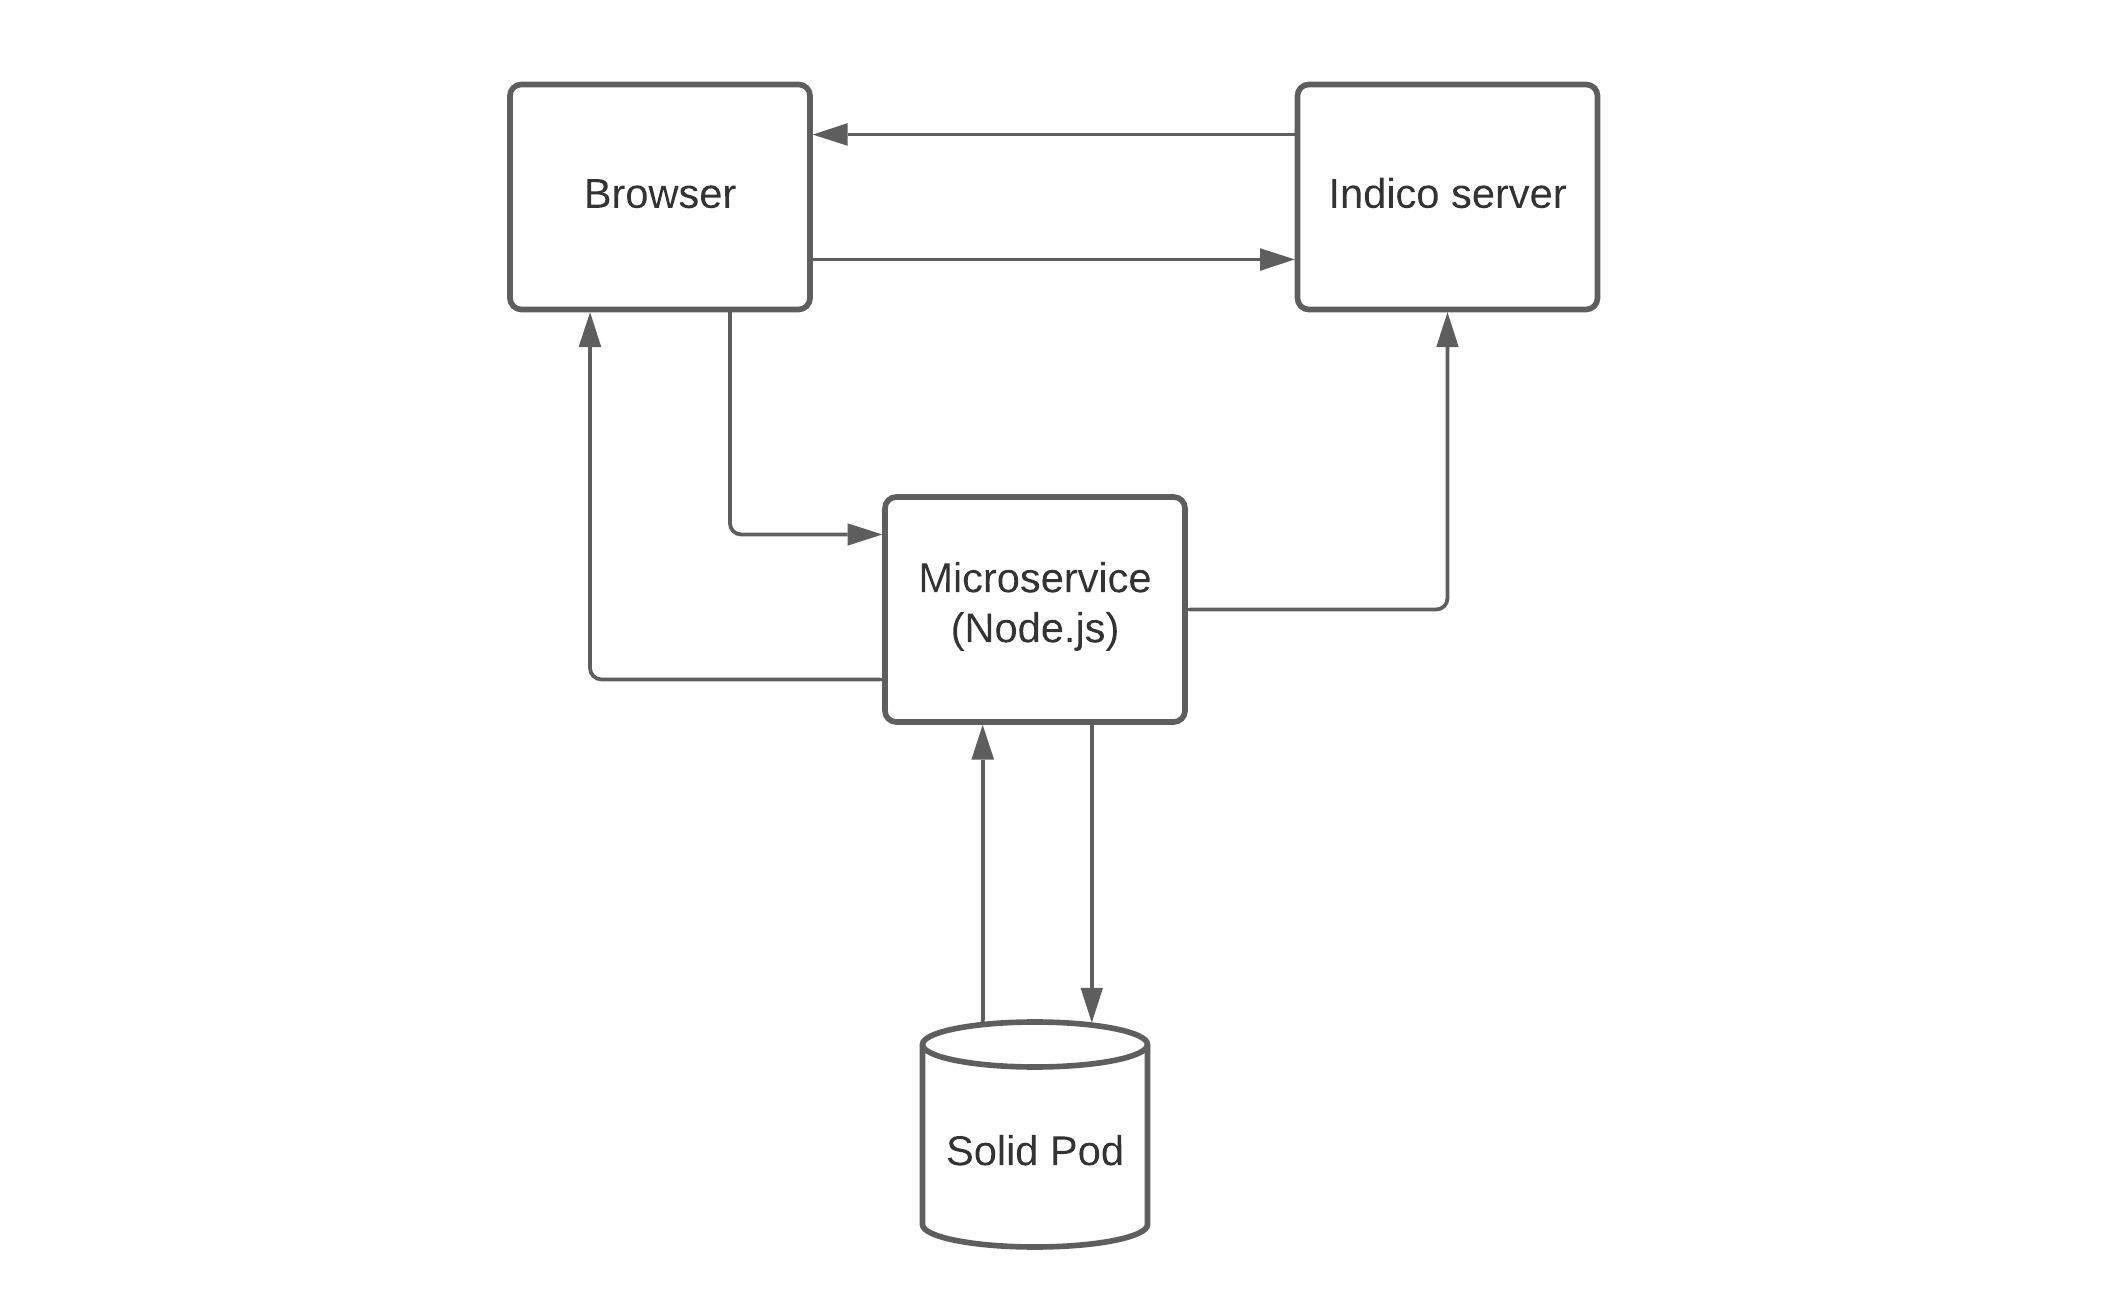
\includegraphics[width=0.8\textwidth]{prototype/graphs/poc-infrastructure-microservice.jpeg}
    \caption{Communication flow for a module developed as a microservice.}
    \label{fig:poc-infrastructure-microservice}
\end{figure}

\paragraph{Server Approach}\mbox{}\\

Goal of the server approach would be just like with the microservice approach to decouple the logic needed to work with Solid from the client and have it run on a server instance. The attractiveness for the server approach would be it could be fully integrated within Indico and be part of its Python code base. The major drawbacks are no direct Solid libraries written in Python exist to allow a seamless integration into the ecosystem.

\begin{table}[!ht]
    \centering
    \begin{tabular}{| l | l |} 
    \hline
     Problem & Solution \\
     \hline
      Language & Python  \\
      Framework & Flask  \\
      Client & -  \\
      Authentication & pyoidc \cite{pyoidc} missing DPoP\\
      RDF & solid-common-vocab-js \cite{solid-common-vocab-js}, rdflib.js \cite{rdflib.js}  \\
    \hline
    \end{tabular}
    \vspace{0.75cm}
    \caption{Existing solutions to problems for a server approach.}
    \label{table:3}
\end{table}

The authentication library pyoidc allows authenticating with \gls{oidc} systems, but is missing a mandatory feature called \gls{dpop}, which is needed to make requests to protected resources on a data pod.

\begin{figure}
    \centering
    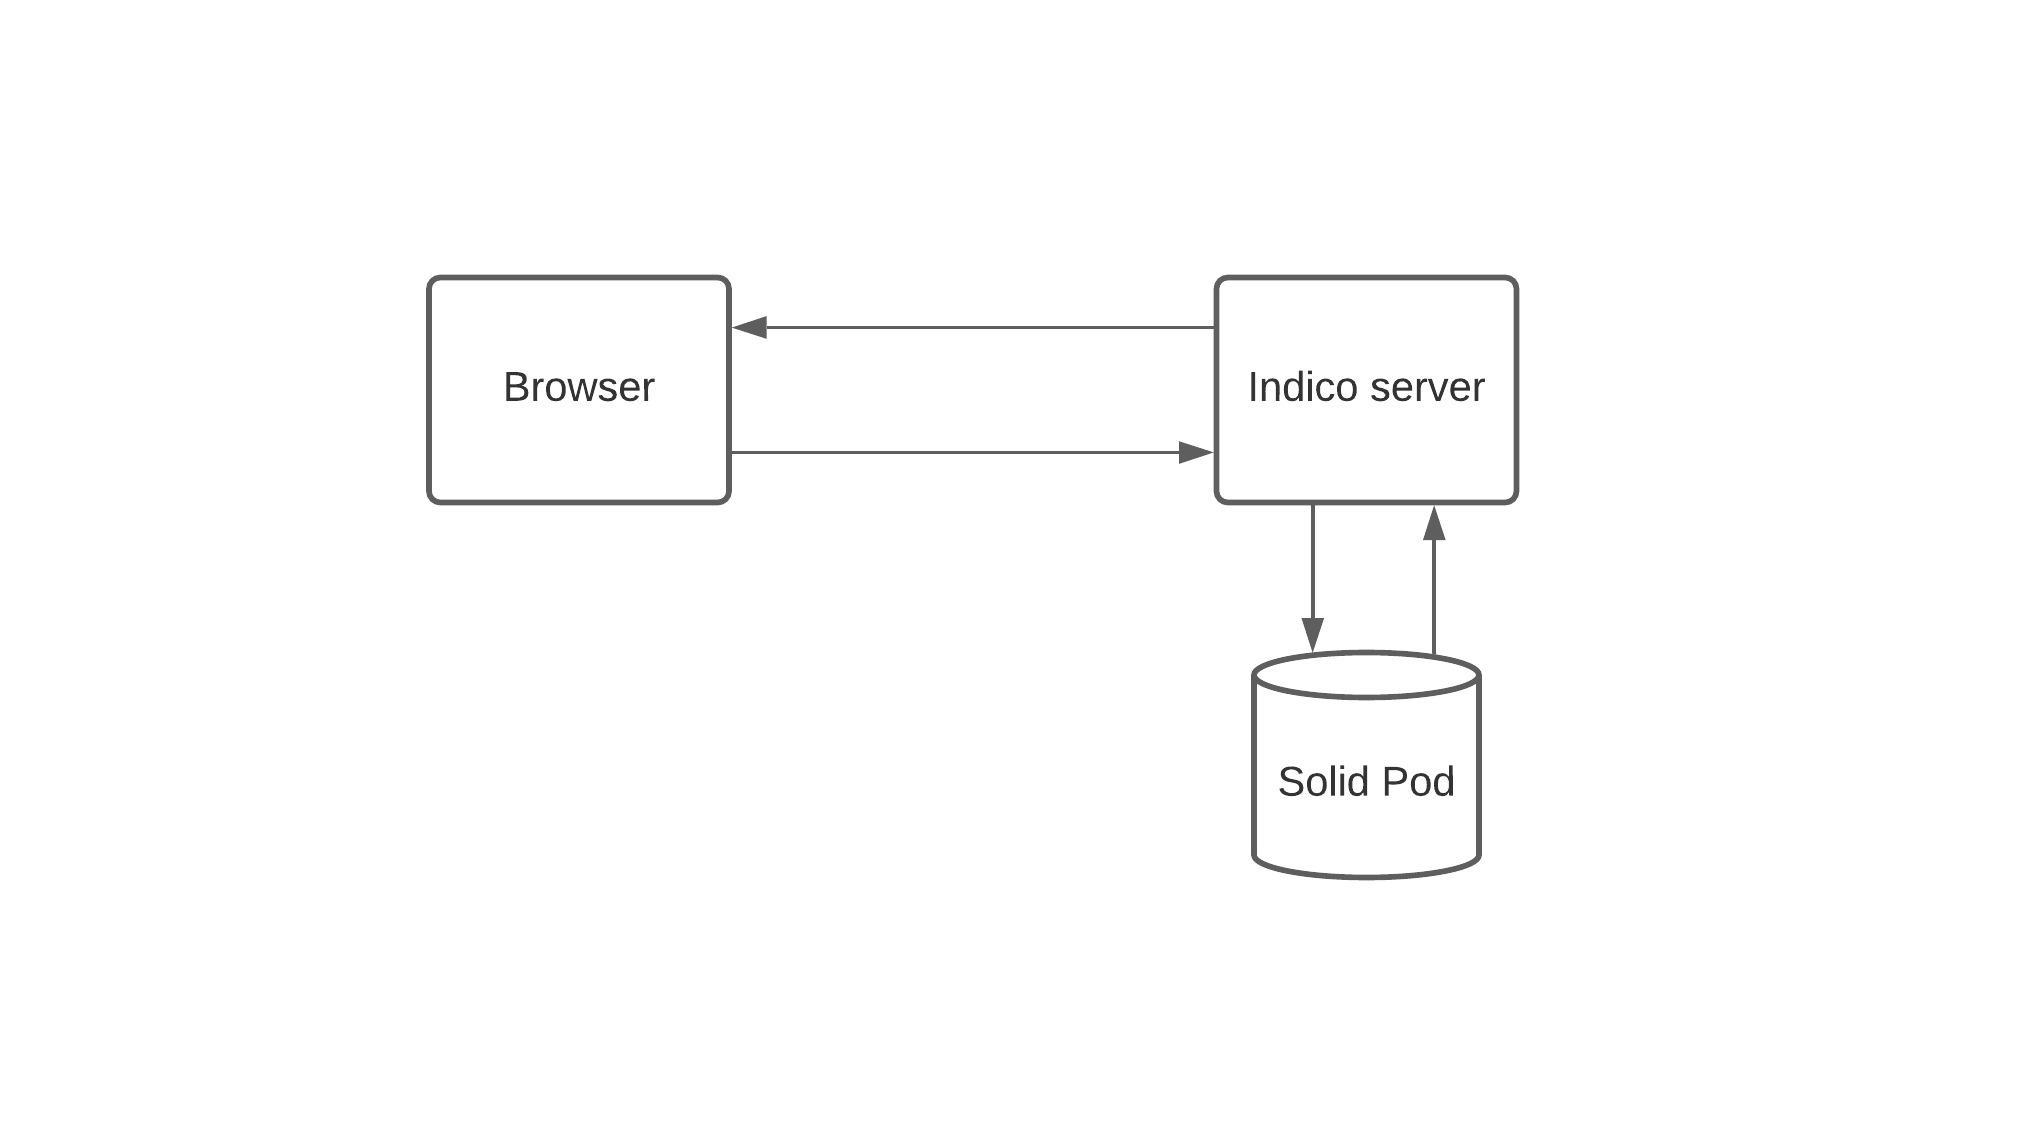
\includegraphics[width=0.8\textwidth]{prototype/graphs/poc-infrastructure-backend.jpeg}
    \caption{Communication flow for a module developed on the server.}
    \label{fig:poc-infrastructure-backend}
\end{figure}

\paragraph{Comparison of the Different Approaches}\mbox{}\\

Benefits from developing the module for the client:

\begin{itemize}
    \item Necessary libraries exist (Major release for all basic Solid flows exist)
    \item Community support
    \item Programming effort for an \gls{mvp} lowest
    \item Documentation on developing Solid apps in JavaScript exist
\end{itemize}

\begin{table}[h!]
    \centering
    \begin{tabular}{| l | p{11cm} |} 
    \hline
     Library & Description \\
     \hline
      solid-client & A client library for accessing data stored in Solid Pods.  \\
      \hline
      solid-client-authn & A set of libraries for authenticating to Solid identity servers:solid-client-authn-browser for use in a browser.solid-client-authn-node for use in Node.js.  \\
      \hline
      vocab-common-rdf & A library providing convenience objects for many RDF-related identifiers, such as the Person and familyName identifiers from the Schema.org vocabulary from Google, Microsoft and Yahoo!  \\
      \hline
      vocab-solid-common & A library providing convenience objects for many Solid-related identifiers.  \\
      \hline
      vocab-inrupt-common & A library providing convenience objects for Inrupt-related identifiers.  \\
      \hline
    \end{tabular}
    \vspace{0.75cm}
    \caption{Existing solutions to problems for a server approach.}
    \label{table:2}
\end{table}

\paragraph{Single Versus Multiple Resource(s) for Comments}\mbox{}\\

Storing the comments in \gls{rdf} can be done in two ways: storing it in one file as a graph with a list of comments, or creating a file for every comment.

\begin{figure}
    \centering
    \begin{subfigure}{.5\textwidth}
      \centering
      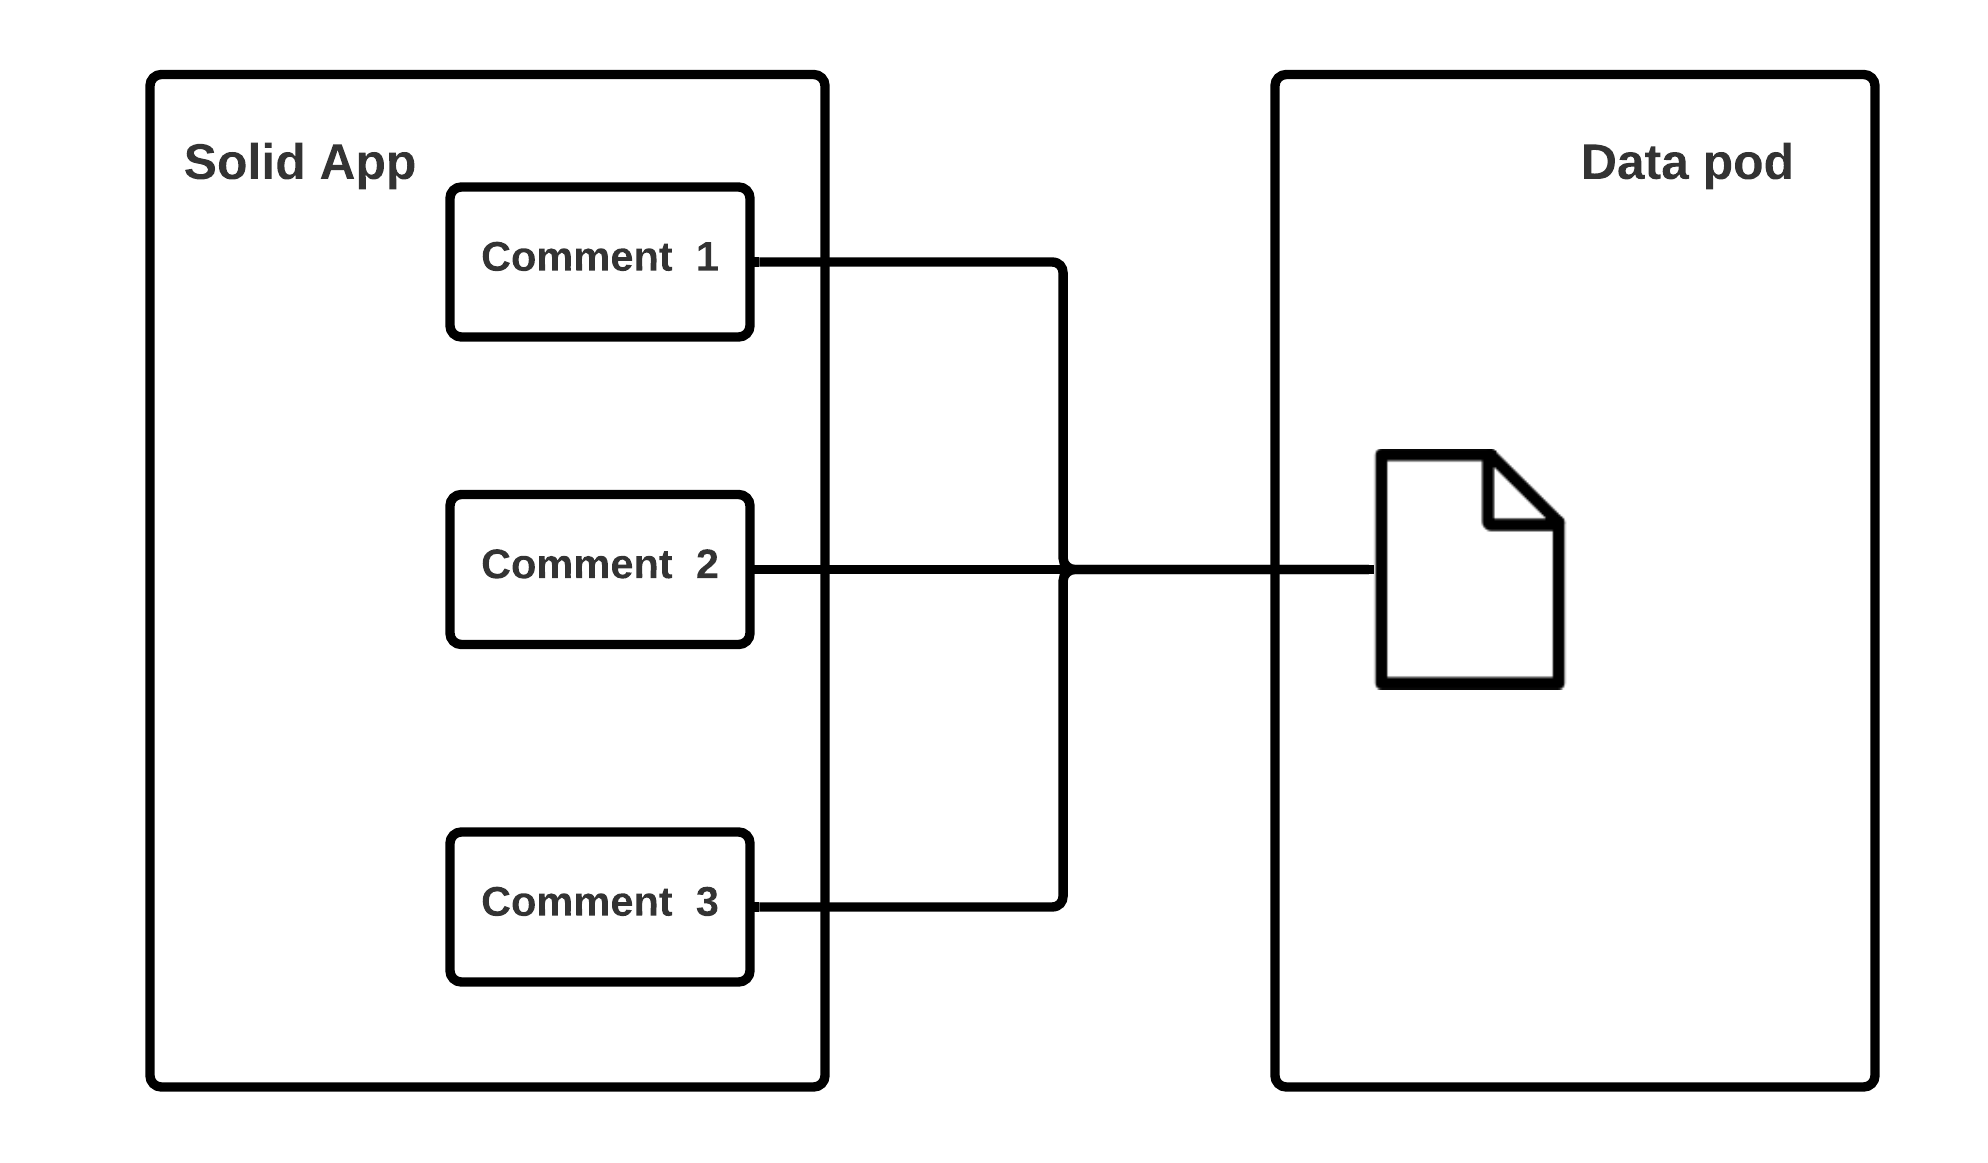
\includegraphics[width=0.7\textwidth]{prototype/graphs/poc-comment-single-resource-comments.png}
      \caption{TODO: caption}
      \label{fig:ppc-comment-single-resource-comments}
    \end{subfigure}%
    \begin{subfigure}{.5\textwidth}
      \centering
      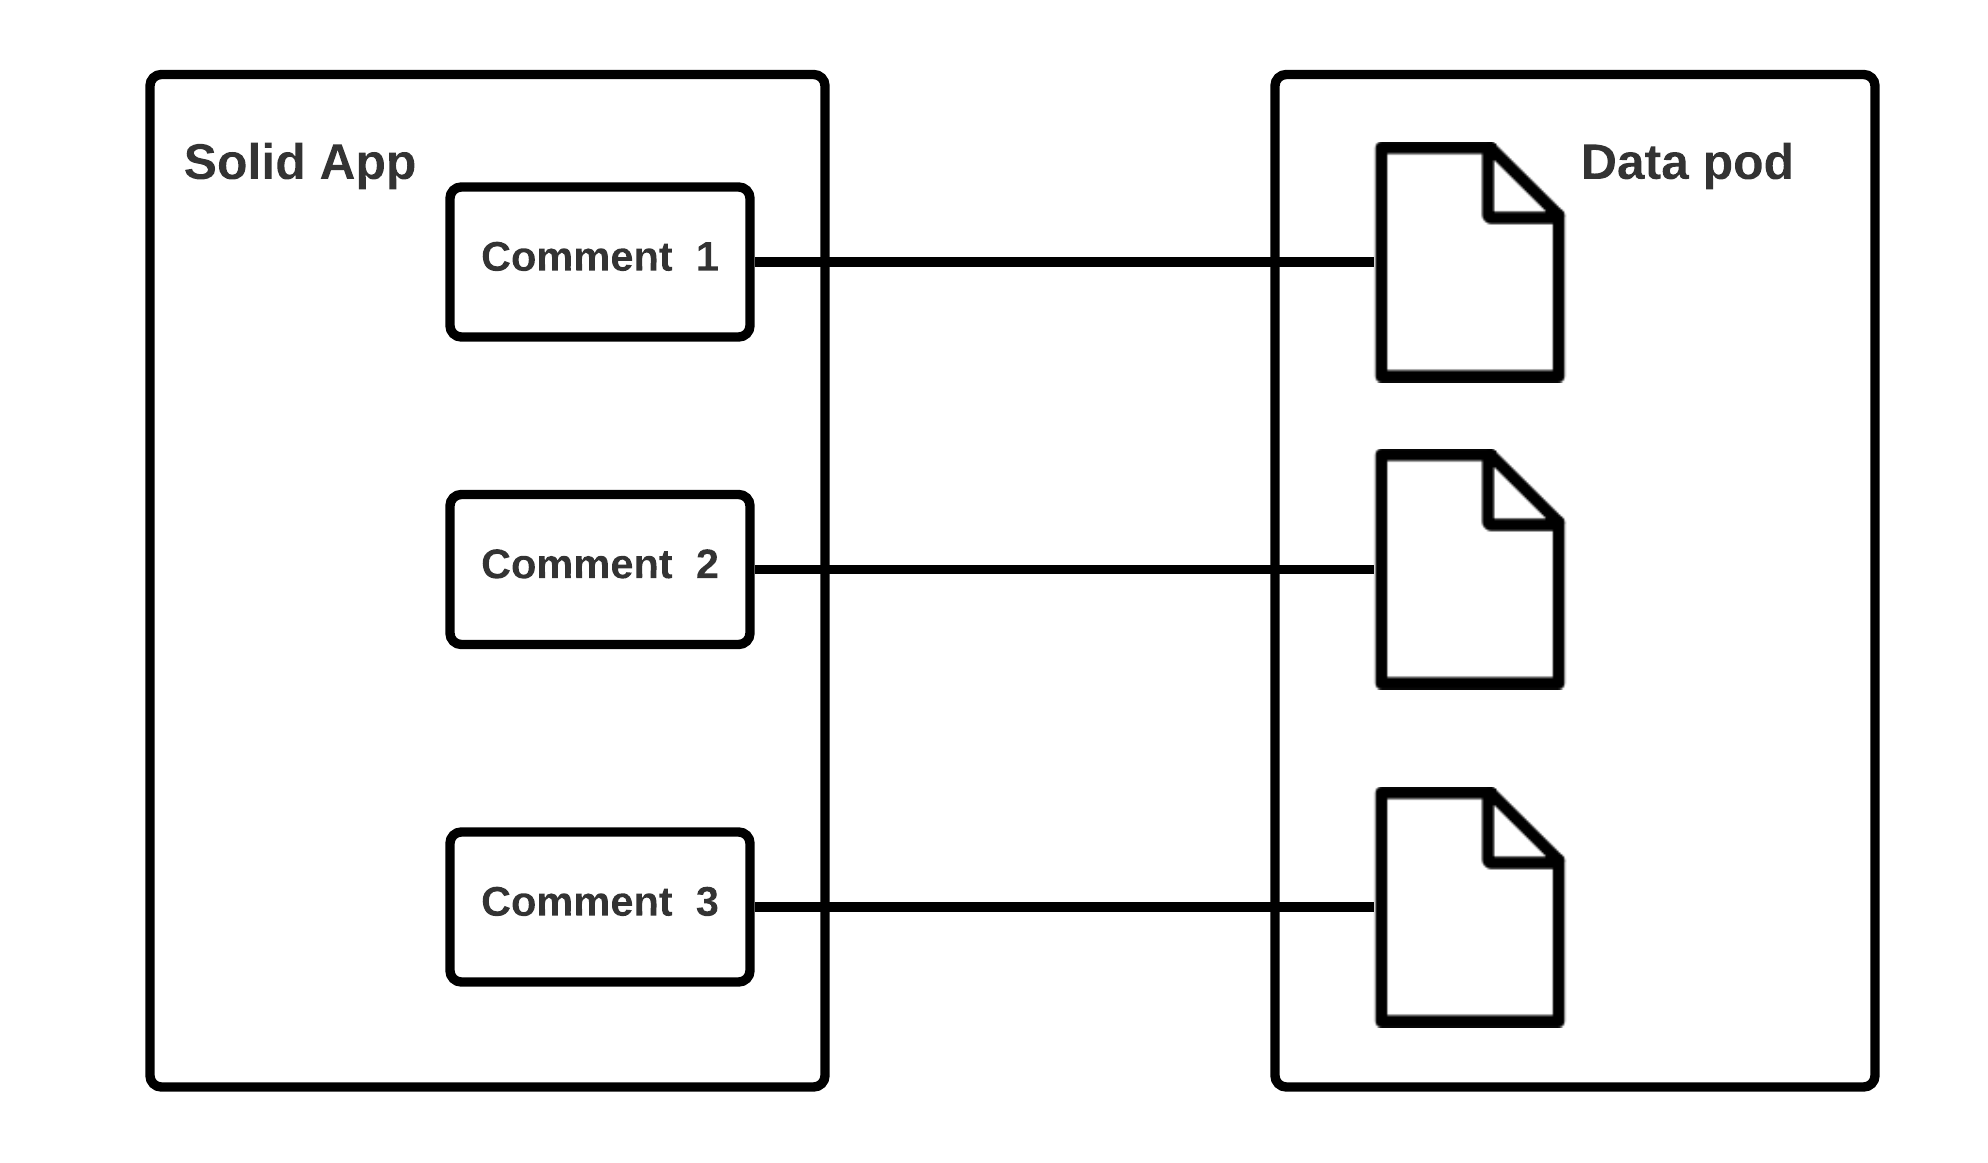
\includegraphics[width=0.7\textwidth]{prototype/graphs/poc-comment-multiple-resources-comments.png}
      \caption{TODO: caption}
      \label{fig:poc-comment-multiple-resources-comments}
    \end{subfigure}
    \caption{TODO: two approaches}
    \label{fig:test}
\end{figure}

When fetching the container with all the comment resources the request returns a Turtle file describing the container, but not the actual content of the contained resources. The misconception of receiving the content as well, was thought to be a problem, as it was assumed an initial request to the container reading its child resources had to be made and then for each resource a request needed to be built to retrieve the resource. This overhead was later disproved as the application where this module is embedded maintains the list of resources to be fetched. Therefore, no manual building of requests to those resources had to be done. The next paragraph also lays out how this design would not work with the protection of the resources.

\paragraph{Protection on Resource}\label{protection-on-resource}\mbox{}\\

Every container and resource in Solid is protected with \gls{wac}, which determines if specific agents, groups, or the world can have read, write, append, or control access. These control access modes are defined in \gls{acl} files. The Solid \gls{acl} inheritance algorithm looks for an \gls{acl} file attached to a specific resource, if it cannot find one it goes recursively up the file hierarchy and looks for \glspl{acl} on the containers.
Indico allows two general types of protection \textit{private} and \textit{public} on its events. Public means open to everyone, no Indico account or any type of authorization is needed to see the event. Whereas private can be as fine-grained as only to specific agents or groups. A comment module is only valuable if the comments can be read by anyone and be written by authorized users.

In order for visitors of a private or public event in Indico to be able to see the comment, the comment’s \gls{acl} needs to allow the public to read the resource. This can be achieved by using the \textit{public} container, which comes with public-read by default on the \gls{nss} or by creating a new container and setting the \gls{acl} with:

\begin{lstlisting}[language=Other,columns=fullflexible, caption={TODO: Label caption}, label={lst:1}]
@prefix acl: <http://www.w3.org/ns/auth/acl#>.
@prefix foaf: <http://xmlns.com/foaf/0.1/>.

# ... Definition for owner

<#example-container-name>
    a acl:Authorization;
    acl:agentClass foaf:Agent;
    acl:accessTo <./>;
    acl:mode acl:Read.
\end{lstlisting}

Every resource in this container is by definition readable by the public -- if not otherwise stated in a more detailed resource \gls{acl}. The above definition even allows the reading of the container’s content, meaning a request to the container would yield a list of resources in the container. This becomes unpleasant if the Indico event is private and the comments for this Indico event should not be read by the world, which is entirely possible, when browsing to the location of a specific data pod and then looking into the public container.

To prevent a random agent to see the contents of a container, the container can be set to private, with the container’s resources to still be public. This would allow everyone provided they have the \gls{url} to browse to the public resource and read it, but not look into the resource’s parent container. To achieve this behavior with \gls{acl}, the container needs to just define its owner and no specific rules for the public, as \gls{wac} comes with a default private access control. Each child resource needs to define an \gls{acl} now, allowing public read.
The container’s \gls{acl} would look like the following with just a owner defined:

\begin{lstlisting}[language=Other,columns=fullflexible, caption={TODO: Label caption}, label={lst:2}]
@prefix acl: <http://www.w3.org/ns/auth/acl#>.

<#owner>
    a acl:Authorization;
    acl:agent <https://janschill.net/profile/card#me>;
    acl:accessTo <./>;
    acl:default <./>;
    acl:mode acl:Read, acl:Write, acl:Control.
\end{lstlisting}

A child resource would allow public read with:

\begin{lstlisting}[language=Other,columns=fullflexible, caption={TODO: Label caption}, label={lst:3}]
@prefix : <#>.
@prefix acl: <http://www.w3.org/ns/auth/acl#>.
@prefix foaf: <http://xmlns.com/foaf/0.1/>.

# ... Definition for owner

:Read
    a acl:Authorization;
    acl:accessTo <test.txt>;
    acl:agentClass foaf:Agent;
    acl:mode n0:Read.
\end{lstlisting}

Another approach and the one implemented after iterating through the previous ones is to have the container’s \gls{acl} resource define a default access mode for its child resources. This way one \gls{acl} only needs to be created on the container and all resources have proper access modes for public read and are not listed publicly in the container’s description.

\begin{lstlisting}[language=Other,columns=fullflexible, caption={TODO: Label caption}, label={lst:4}]
@prefix acl: <http://www.w3.org/ns/auth/acl#>.
@prefix foaf: <http://xmlns.com/foaf/0.1/>.
@prefix target: <./>.

:ReadDefault
    a acl:Authorization;
    acl:default target:;
    acl:agentClass foaf:Agent;
    acl:mode acl:Read.
\end{lstlisting}

\paragraph{Preventing Resources From Unwanted Discovery}\mbox{}\\

With the resources having proper access modes but being publicly readable a simple naming convention of taking the \gls{iso} 8601 string and using it as a filename for the resources created on the data pod does not suffice -- even though it is a good strategy when looking for a reliable naming convention to prevent duplication. Considering performance improvements such as pagination for future iterations of the module, which would require some sort of iterative indication, a combination of randomness, but also a order indicator it was settled for using \gls{uuid} plus the \gls{iso} 8601 string to form a filename.

Other ideas included hashing a random string with the timestamp to generate non-guessable filenames. The filename would need to use the same hash function to decipher the filename to figure out when the comment was generated. \gls{uuid} is a reliable and easy to use system to generate \textit{truly} globally unique strings. 

\paragraph{Modification of Resource From Data Pod}\mbox{}\\

\paragraph{Mitigation of Spam}\mbox{}\\

Enabling user input in form of comment module without application authentication is a gateway to spam. Even though authentication with a Solid \gls{idp} is necessary, it does not hinder a malicious actor to create a multitude of Solid accounts and spam into the application. In the first iteration of the module only Solid authentication was integrated into the module and would therefore allow anyone with a Solid account to post comments and thus also spam the Indico event theoretically. In a second iteration of the module another authentication layer was added to mitigate spam from outside of Indico. For \gls{cern}’s use-case an authenticated Indico session was enough. This adds an extra step to the comment process and it is ensured only registered Indico users can comment.

\paragraph{Giving Application Full Control of Data Pod}\mbox{}\\

To create or change programmatically \glspl{acl} requires \textit{control} access to the container. By default \gls{nss} asks for the permissions when authenticating for the first time in the \gls{solidoidc} flow between the \textit{solid-comment} module and Solid \gls{idp}. The permissions granted to the application are on the root container of the data pod. Meaning, giving an application control access allows the application to read, write, change \glspl{acl} on the entire data pod. This is obviously troubling, as a simple application as a commenting module need to have control access to set the needed \glspl{acl} for the containers and resources it creates.

The current implementation has not a built-in solution, but one way of solving it, is the use of an application launcher, which is an application itself with full control access and then limits the access controls of the \textit{solid-comment} module by creating a dedicated container for it and setting the needed \gls{acl} for this specific container only.

\subsubsection{Integration with Indico}

The need for integration with Indico is twofold: serving the module to the client and being the provider to the list of references to the comments that have been posted on a specific event.

\paragraph{Storing Reference to Comments in Indico}\mbox{}\\

\paragraph{Enforce Authenticated Session For Posting Comments}\mbox{}\\

\subsubsection{Evaluation}



\paragraph{System Description}\mbox{}\\

The system aims at enabling commenting in web application with decentralized storage on data pods. The system in the context of Indico aims at allowing Indico users with a data pod to comment on specific Indico events.

\paragraph{Features}\mbox{}\\

\begin{enumerate}
    \item A user with a Solid account can authenticate with their Solid \gls{idp}
    \item A user can compose a text which is stored on their data pod
    \item A user can see other users’ comments
\end{enumerate}

\paragraph{User of the System}\mbox{}\\

There are two types of users in the system. The one interested in the application where this comment module is implemented and is either solely interested in also looking at the comments or also interested in commenting. The other type of user is the administrator of the application where this system is implemented in. This type of user is interested in keeping the tone of comments to their desire and not allow any misuse.

\paragraph{Context Diagram}\mbox{}\\

\begin{figure}[H]
    \centering
    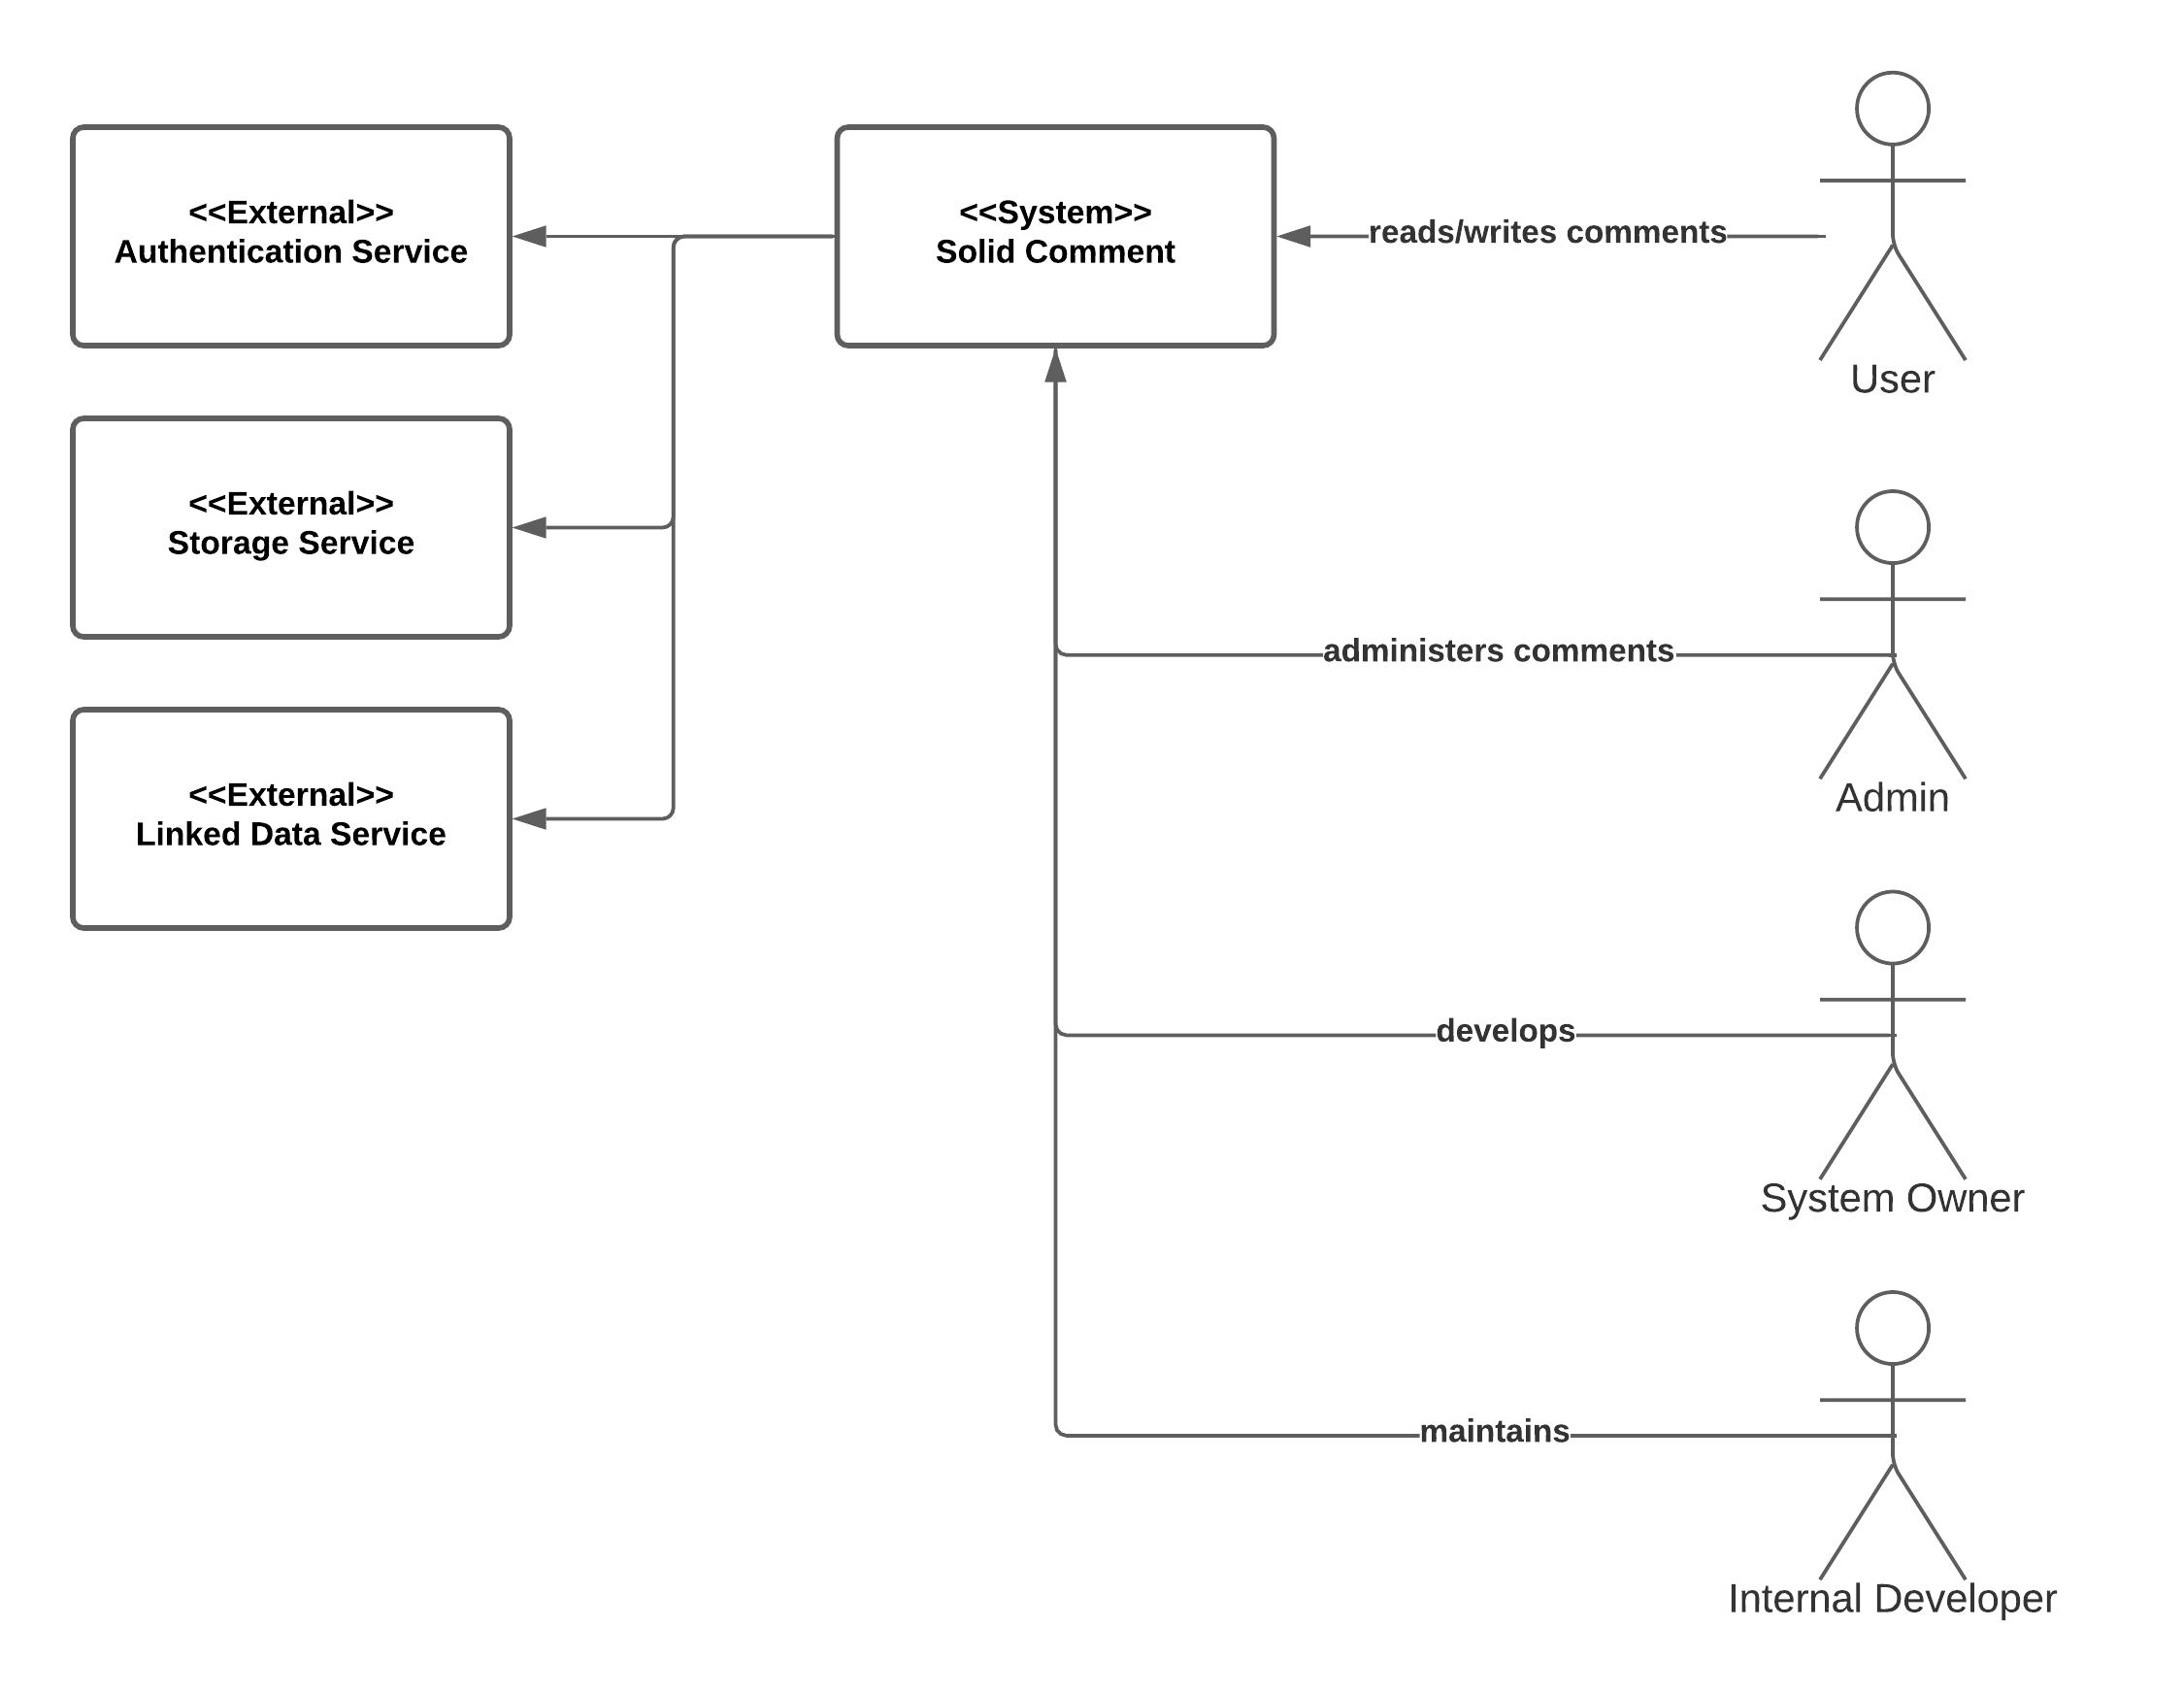
\includegraphics[width=0.8\textwidth]{prototype/graphs/poc-comment-context_diagram.png}
    \caption{Context diagram showing users and external services of system.}
    \label{fig:poc-comment-context_diagram}
\end{figure}

\paragraph{Sequence Diagram}\mbox{}\\

\begin{figure}[H]
    \centering
    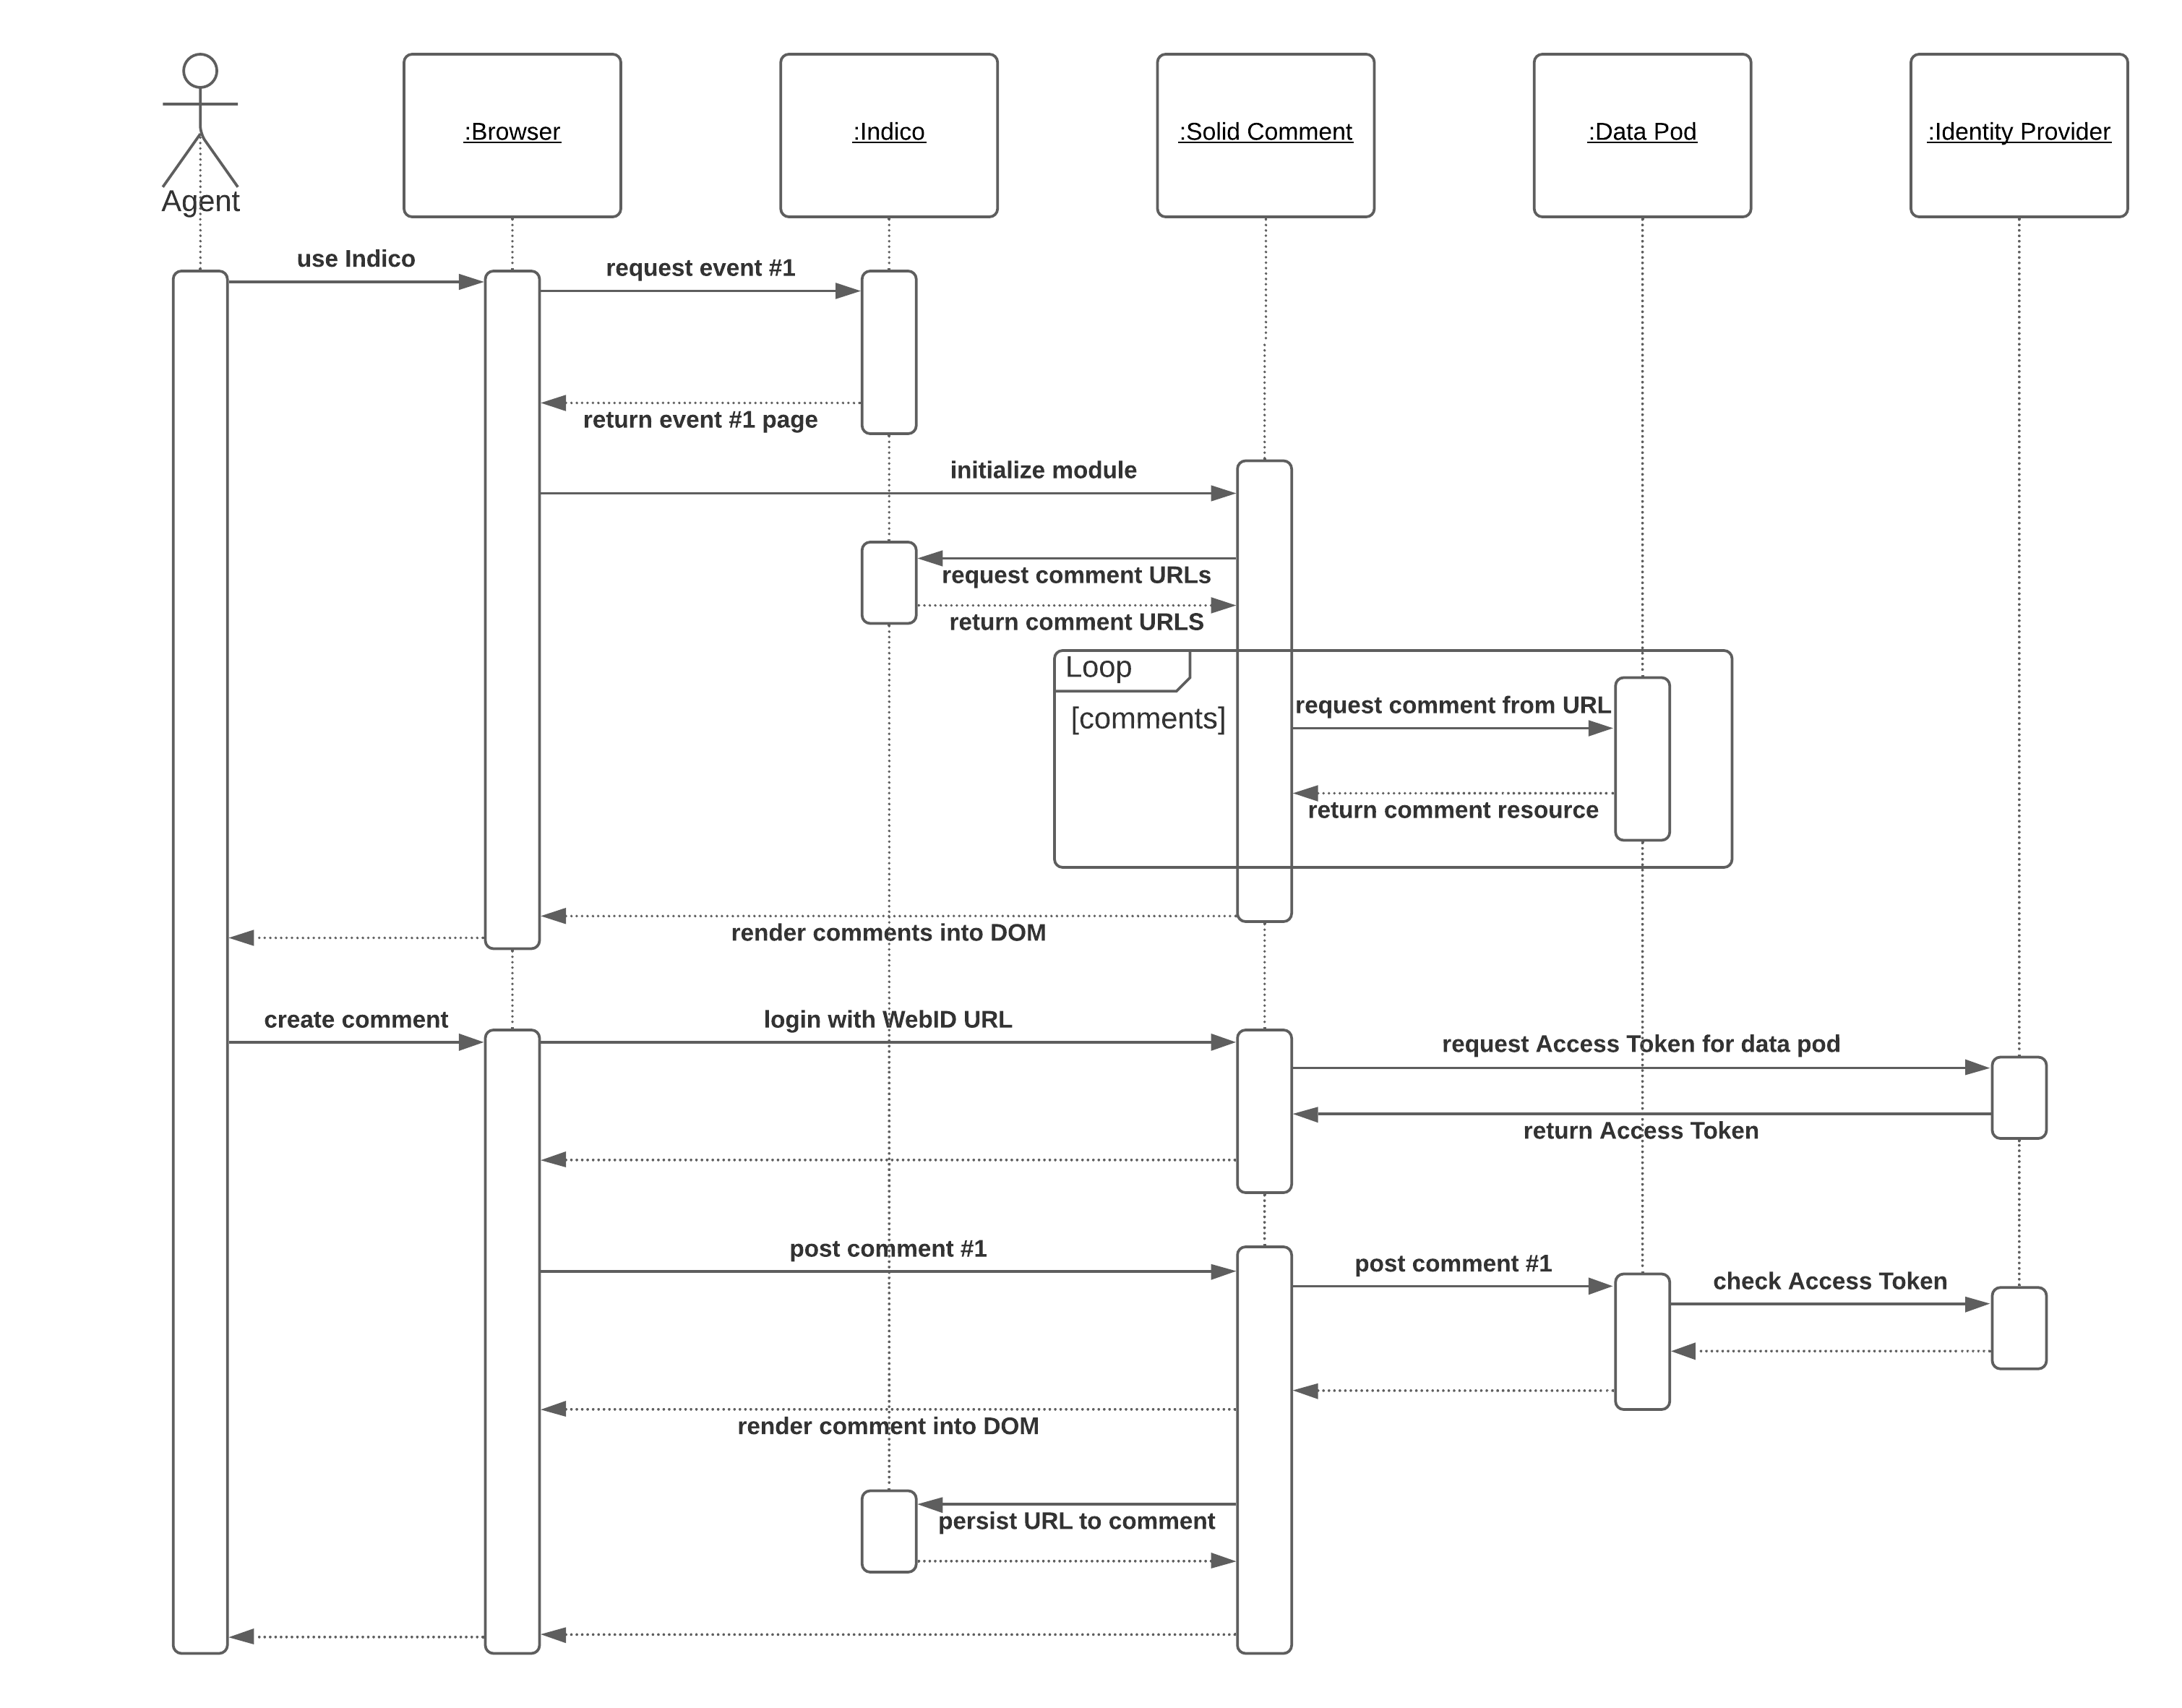
\includegraphics[width=\textwidth]{prototype/graphs/poc-comment-sequence_diagram.png}
    \caption{Sequence diagram showing the sequential process through posting a comment.}
    \label{fig:poc-comment-sequence_diagram}
\end{figure}

\paragraph{Stakeholders}\mbox{}\\

A few stakeholders are involved which
\paragraph{Drivers}
\paragraph{Metrics}

\begin{enumerate}
    \item Security
    \item Performance
    \item Usability
\end{enumerate}

\paragraph{Levels}\mbox{}\\



\paragraph{Components}\mbox{}\\

\paragraph{Scenarios}\mbox{}\\

\begin{enumerate}
    \item A user who has commented deletes their comment in their data pod
    \item A user who has commented deletes their data pod
    \item A user uses a script to generate a large number of comments
    \item A user creates a comment with a \gls{xss} attack
\end{enumerate}


\subsubsection{Analysis}

* EventProxy is not scalable, when comments are sent at the same time could be overwritten
* log IP and blog on spam
* extra layer api to cache comments, performance and security against IP logging
* one pod sends different content to users depending on their location

\subsection{POC 2: Auto-Complete for Conference Registration in Indico}

\subsubsection{Design}

TODO:
1st iteration, save data in pod
2nd iteration, only pull data from pod

\paragraph{Modification of Resource From Data Pod}\mbox{}\\

\paragraph{Payment on Input Fields}\mbox{}\\

\paragraph{Performance of Large Conference}\mbox{}\\

\paragraph{Availability of Crucial User Data}\mbox{}\\

\subsubsection{Integration With Indico}

\paragraph{Bind to Dynamically Created Form}\mbox{}\\

\subsubsection{Evaluation}

\paragraph{System Description}\mbox{}\\
\paragraph{Context Diagram}\mbox{}\\
\paragraph{Stakeholders}\mbox{}\\
\paragraph{Drivers}\mbox{}\\
\paragraph{Metrics}\mbox{}\\
\paragraph{Levels}\mbox{}\\
\paragraph{Components}\mbox{}\\

\subsubsection{Analysis}

\subsection{Deployment of Indico Instance}

% \newpage
% \section{Comparison of Solid and Indico Design Principles}

\newpage
\section{Challenges, Advantages, and Gaps of Existing Solid Solutions versus CERN Ones}

* 
* Encryiption -> hosting on premise
* Hosting on premise -> high involvement with the servers
* Solid UI challenges
* Commercial and open-source not perfectly hand in hand
* Not many applications in Solid ecosystem
    * no sophisticated to say the least
    * the closest LiqidChat makes heavy use of an API
\newpage
\section{Continuation in the CERN-Solid Collaboration}

With the two prototypes developed, integrated into Indico, and deployed to a running instance and showing a working solution with Solid principles in Indico, how can \gls{cern} proceed with its collaboration attempt? In the following, the two fields of Solid specification implementations and Solid apps shall be looked at and debated what \gls{cern}'s role in the future of Solid can be.

\subsection{Solid Servers}

The in \cite{cern-solid-investigation-spec} identified Solid implementations remain where they were when composing the research paper \cite{cern-solid-investigation-spec}. A lot of development has happened for the \gls{css}, but it is still in a minor release version and therefore not yet deployed and switch out with \gls{nss} on the public solidcommunity.net domain. This is expected to happen as soon the developers trust the state of \gls{css} to facilitate at least the functionality of \gls{nss} and the tooling is in place to transfer all existing data pods currently hosted on the web server. No publicly communicated date has been set in stone for this to occur but it can be assumed to happen this year or next. The Solid specification, on the other hand, has a clearly defined completion date of 30.06.21 \cite{solid-tr}. Once the technical reports are completed -- but of course remain in the state of a living standard -- it can be expected to ease the development process in the Solid ecosystem, as no significant changes in the specification mean no critical new features need to be developed or supported by the server developments.

The \gls{nss} is maintained by a small team of unfunded open-source developers and can only fix critical bugs and keep the dependencies up-to-date. It is still the most used Solid implementation and recommended data pod solution in conjunction with one of the providers, namely solidcommunity.net \cite{solid-community}.

\gls{cern} has a number of options in its continuation with Solid servers in their current status.

\begin{enumerate}
    \item Outstanding solution through solidcommunity.net
    \item Integration with CERNBox
    \item Sandboxed \gls{css}
    \item Develop own server solution
\end{enumerate}

\paragraph{Outstanding Solution}\mbox{}\\

The usage and testing of the \glspl{poc} required a WebID and a data pod. Through extensive research and careful considerations, it was concluded and recommended to all \gls{poc} participants to obtain the necessities through solidcommunity.net. The Solid Community is currently the most attractive data pod provider through its physical hosting in the \gls{uk} and openness regarding data usage and usage of \gls{nss} the go-to open-source Solid server solution. \gls{cern}, by policy, opts for data storage in European locations based on \gls{oc11} \cite{oc11}] and \gls{gdpr} \cite{gdpr}, and that all data are merely used to provide its services \cite{policy-cern-server}. Storage locations outside Europe can be possible only if there is a clear justification officially approved by the \gls{cern} \gls{odp}. This is also a reason why a hosted instance through Inrupt \cite{inrupt} not acceptable. Not to mention the expected cost of such a service. An outstanding solution also gives away control over the running version of the Server implementation. As of now most data pod providers run the \gls{nss}, but might switch over to \gls{css} -- which is desirable but could bring new challenges. Even though a server implementation can only be called a Solid server when it adheres to the Solid specification, which can be tested by an \gls{ists} \cite{solid-test-suite}, which also means when the specification is followed, features should be equally supported and implementations should allow interoperability. This has been proven to be difficult when looking at the several browsers, which are all implementing the \gls{http}, \gls{html}, and \gls{uri} standards (and many more specifications) but are all behaving slightly differently. This might be due to missing resources to stay up to date with feature development, or contrasting interpretations of the specifications. These risks will always endure and hence bring challenges.
\vspace{0.5cm}
\paragraph{Integration With CERNBox}\mbox{}\\

\gls{cern} uses CERNBox \cite{cernbox} to provide personal cloud storage to all \gls{cern} users to host and share files. The service is based of ownCloud \cite{owncloud} and hosted on \gls{cern} premise. In 2016 Nextcloud \cite{nextcloud} was formed from a fork of the open-source core software of ownCloud. PDS Interop \cite{pds-interop}, a collective of open-source developers, has developed a Nextcloud \cite{nextcloud} plugin to make the file hosting service Solid compatible. A Nextcloud server with the Solid plugin enabled passes currently the complete \gls{ists}. The integration with a running Nextcloud instance is as easy as installing the plugin through the web interface of Nextcloud.

An integration with CERNBox seems to be a suitable option, provided resources are attributed for taking care of operational requirements and security preoccupations. Adding the Solid implementation into its own cloud storage infrastructure means the CERNBox administrators now also have to administer the Solid Nextcloud plugin. Performance issues due to the thousands of CERN users should be studied in advance. A possibility could be to only enable it for a subset of users to test the integration. Resources for these steps would have to be planned. Most importantly, the attack surface increased by enabling a plugin that includes an extra sharing functionality would have to be analyzed.
\vspace{0.5cm}
\paragraph{Sandboxed \gls{css}}\mbox{}\\

A less risky solution would be to use a sandboxed Solid implementation, such as \gls{css}. Once \gls{css} is released under a major version it could be deployed to self-contained OpenStack VM instances and then run as a new file storage system. This might seem redundant, considering \gls{cern} is already running a cloud storage system with CERNBox, but the added risk is much lower to infiltrate an existing system. The new \gls{css} deployments could solely be used for Solid related file storage and sharing and then incrementally be more integrated with existing \gls{cern} solutions. Even though the complexity might not be as high as with the installation through the Nextcloud plugin in CERNBox it still requires administrative work to keep the deployments running and updating \gls{css} regularly. Further, to even add more value and usability to this integration the \gls{css} could be used with the \gls{cas}. Meaning, instead of identifying with an external \gls{idp}, the \gls{cern} users could authenticate with their existing \gls{cern} accounts using \gls{cas}, which would need to be extended to also provide WebIDs.

Open-source and community-owned software brings a lot of advantage but also needs to be tread lightly. Software as this always relies on independent developers to fix bugs, develop features, which will not happen as fast when using a product with \glspl{sla}. A motivator for \gls{cern} to get involved with the development of open-source Solid services.
\vspace{0.5cm}
\paragraph{Own Server Solution}\mbox{}\\

Because Solid is an open standard and allows free development of own solutions it is always a possibility to develop a \gls{cern} Solid server from scratch. This is from all solutions the most ambitious one and least recommended, as it demands too many resources and a sophisticated solution through \gls{css} is almost release, which would benefit from additional given resources.

\subsection{Solid Applications}

Uncertainties in the adoption of a CERN Solid server do not help to advocate the usage of Solid applications or even the development of new Solid services. The \glspl{poc} have shown realistic use-cases for decentralized data storage. The architectural evaluation has shown the maturity, but also the flaws that would need to be tackled in order for them to be adopted into the production instance of Indico at \gls{cern} and then it also needs to be analyzed if those \glspl{poc} would even find users or it would be just a dead feature. Indico has also been established to not be the perfect candidate for a complete Solid overtake in its architecture. Therefore, less complex software at \gls{cern} might be a better target for further Solid-based developments. One prospect is the \gls{cern} Slides' App \cite{cern-slides}, which is a web application recently developed as part of a student project and is in production-ready quality and planned to be used as a main slides maker for \gls{cern} users. A possibility for \gls{cern} to remain present in the Solid ecosystem is to further the development of the Slides' App and even make it Solid compatible. The final resource combining all slides into a single presentation could be stored in a data pod, and even further thought all the information on the slides could be connected to resources from data pods and thus leveraging a decentralized approach to data management. Everything would be connected, could be reused, and would be completely interoperable. Information could still come from non-\gls{rdf} resources but could be transformed to \gls{rdf} upon entry. Resulting in an attractive hybrid application, that could be used without the need of a data pod or WebID, but would still find users as it is a wanted software at \gls{cern} and would bring the decentralized resource management to the ones who want to use it.

Another minor idea in the field of application development is based from the second \gls{poc} the autocomplete module, that the existing \gls{cern} application could be enriched by using more structured data concepts in their code. As an example attache the \gls{html} \texttt{autocomplete} attribute to known input fields. Add more common input fields to allow the pre-definition of semantic structure on them. This way the forms can be reasoned about easier by machines, but this effort should not be limited to \gls{html} forms and can be extended to all sorts of fields where Schema.org has a description for.

\subsection{Recommendation}

A recommendation based on the previous two talked about fields of server implementation and application development for \gls{cern} is as follows.

The current efforts from \gls{cern} are rather limited in resources, general interest is present, but many factors hinder further active involvement with Solid. A public communication channel used to share milestones in the investigation is left unread. Announcements and call for testings of the \glspl{poc} in \gls{cern} internal email groups reaching hundreds of \gls{cern} users are met with participation, compliments, and comments, but still small in number. A presentation given at the HEPiX \cite{hepix} was well received by international Information Technology staff, from High Energy Physics and Nuclear Physics laboratories and institutes. So, a general curiosity exists, and a few enthusiasts are awaiting a Solid-like project to be supported by \gls{cern}, but it seems more generally that \gls{cern} is interested in an observing position as of now. University students are currently sought to work on the follow-up \gls{cern}-Solid project \cite{cern-slides}. This will be beneficial for \gls{cern} for continuing further understanding of the Solid ecosystem and receive the latest developments in server implementations, specification evolution, and new exciting Solid apps. It will also benefit the students for their studies and experience in dealing with complex projects and environments. Once the Solid ecosystem has matured enough and has shown through other Solid app developments the possibilities and innovations with Solid, \gls{cern} can reevaluate its position and consider participating more actively by either Solid app development or hosting Solid pods for its users.


\newpage
\chapter{Conclusion}
% \setcounter{section}{0}




* Solid lives through the community, when only one company does the implementation it will not thrive
* vicious cycle
* 

Solid from the community, for everyone
start by the community
get going, but breakthrough takes more -> CERN

community <-> company
not just one company it won't thrive

software needs to be rethought
major challenges:
    usability
    performance
    describing the world in Linked Data, can the data of the complex world be described for by machines?
it takes entities as CERN to not let commercial companies built the products, otherwise Solids futures might be at stake? (a bit harsh)

solid is still experimental and needs a lot of attention from developers
startups are good
the more the merier
the community needs to remain as a driver
high profile people help, but cannot be the motivator

build better and hybrid products for people where they might not even realize the decentralized benefits

challenge the known
\newpage
\printglossary[type=\acronymtype]
\newpage
\printglossary
\newpage
\printbibliography
\end{document}
